\documentclass[]{book}
\usepackage{lmodern}
\usepackage{amssymb,amsmath}
\usepackage{ifxetex,ifluatex}
\usepackage{fixltx2e} % provides \textsubscript
\ifnum 0\ifxetex 1\fi\ifluatex 1\fi=0 % if pdftex
  \usepackage[T1]{fontenc}
  \usepackage[utf8]{inputenc}
\else % if luatex or xelatex
  \ifxetex
    \usepackage{mathspec}
  \else
    \usepackage{fontspec}
  \fi
  \defaultfontfeatures{Ligatures=TeX,Scale=MatchLowercase}
\fi
% use upquote if available, for straight quotes in verbatim environments
\IfFileExists{upquote.sty}{\usepackage{upquote}}{}
% use microtype if available
\IfFileExists{microtype.sty}{%
\usepackage{microtype}
\UseMicrotypeSet[protrusion]{basicmath} % disable protrusion for tt fonts
}{}
\usepackage[margin=1in]{geometry}
\usepackage{hyperref}
\hypersetup{unicode=true,
            pdftitle={Animal Disease Surveillance, AFBI},
            pdfauthor={Agri-Food and Biosciences Institute},
            pdfborder={0 0 0},
            breaklinks=true}
\urlstyle{same}  % don't use monospace font for urls
\usepackage{natbib}
\bibliographystyle{apalike}
\usepackage{longtable,booktabs}
\usepackage{graphicx,grffile}
\makeatletter
\def\maxwidth{\ifdim\Gin@nat@width>\linewidth\linewidth\else\Gin@nat@width\fi}
\def\maxheight{\ifdim\Gin@nat@height>\textheight\textheight\else\Gin@nat@height\fi}
\makeatother
% Scale images if necessary, so that they will not overflow the page
% margins by default, and it is still possible to overwrite the defaults
% using explicit options in \includegraphics[width, height, ...]{}
\setkeys{Gin}{width=\maxwidth,height=\maxheight,keepaspectratio}
\IfFileExists{parskip.sty}{%
\usepackage{parskip}
}{% else
\setlength{\parindent}{0pt}
\setlength{\parskip}{6pt plus 2pt minus 1pt}
}
\setlength{\emergencystretch}{3em}  % prevent overfull lines
\providecommand{\tightlist}{%
  \setlength{\itemsep}{0pt}\setlength{\parskip}{0pt}}
\setcounter{secnumdepth}{5}
% Redefines (sub)paragraphs to behave more like sections
\ifx\paragraph\undefined\else
\let\oldparagraph\paragraph
\renewcommand{\paragraph}[1]{\oldparagraph{#1}\mbox{}}
\fi
\ifx\subparagraph\undefined\else
\let\oldsubparagraph\subparagraph
\renewcommand{\subparagraph}[1]{\oldsubparagraph{#1}\mbox{}}
\fi

%%% Use protect on footnotes to avoid problems with footnotes in titles
\let\rmarkdownfootnote\footnote%
\def\footnote{\protect\rmarkdownfootnote}

%%% Change title format to be more compact
\usepackage{titling}

% Create subtitle command for use in maketitle
\newcommand{\subtitle}[1]{
  \posttitle{
    \begin{center}\large#1\end{center}
    }
}

\setlength{\droptitle}{-2em}

  \title{Animal Disease Surveillance, AFBI}
    \pretitle{\vspace{\droptitle}\centering\huge}
  \posttitle{\par}
    \author{Agri-Food and Biosciences Institute}
    \preauthor{\centering\large\emph}
  \postauthor{\par}
      \predate{\centering\large\emph}
  \postdate{\par}
    \date{14 December, 2018}

\usepackage{booktabs}
\usepackage{booktabs}
\usepackage{longtable}
\usepackage{array}
\usepackage{multirow}
\usepackage[table]{xcolor}
\usepackage{wrapfig}
\usepackage{float}
\usepackage{colortbl}
\usepackage{pdflscape}
\usepackage{tabu}
\usepackage{threeparttable}
\usepackage{threeparttablex}
\usepackage[normalem]{ulem}
\usepackage{makecell}

\begin{document}
\maketitle

{
\setcounter{tocdepth}{1}
\tableofcontents
}
\chapter*{}\label{section}
\addcontentsline{toc}{chapter}{}

\chapter{Introduction}\label{intro}

AFBI provides an animal disease surveillance and diagnostic service for
the Northern Irish farming industry. Passive (scanning) surveillance is
carried out by collecting and analysing data from post mortem and
clinical samples submitted to the Omagh and Stormont laboratory sites of
the Disease Surveillance and Investigation Branch (DSIB) of AFBI.
Analysis of this data assists in establishing baselines for incidence of
endemic disease, facilitating the recognition of new and emerging
diseases and allowing the rapid identification of changing trends in
disease prevalence. This will allow evidence based decision making
regarding control by veterinary providers and at a national level.

\chapter{Cattle Diseases}\label{cattle-diseases}

\begin{center}\rule{0.5\linewidth}{\linethickness}\end{center}

\section{Neonatal Calves (0-1 months)}\label{neonatal-calves-0-1-months}

As in previous years, enteric infections were the most frequently
diagnosed cause of death for this age group in 2017 in Northern Ireland
(see below breakdown on bovine neonatal enteritis). Failure of passive
transfer of maternal immunity was detected in 65\% of blood samples
tested using the ZST (zinc sulphate turbity test) from calves aged less
than 10 days, highlighting the importance of good colostrum management.
This year respiratory infections were the second most commonly diagnosed
cause of death for this age group.

\begin{table}

\caption{\label{tab:unnamed-chunk-6}The conditions most frequently diagnosed on *post-mortem* examinations of  neonatal calves (0-1 months) in 2017, (n= 610 )}
\centering
\begin{tabular}[t]{l|r|r}
\hline
Category & No. of cases & Percentage\\
\hline
Enteric infections & 254 & 41.6\\
\hline
Respiratory infections & 89 & 14.6\\
\hline
Nutritional / metabolic conditions & 50 & 8.2\\
\hline
Septicaemia / toxaemia & 47 & 7.7\\
\hline
Navel ill / Joint ill & 43 & 7.0\\
\hline
Other diagnoses & 36 & 5.9\\
\hline
Salmonellosis & 23 & 3.8\\
\hline
Diagnosis not reached & 16 & 2.6\\
\hline
Cardiovascular system & 10 & 1.6\\
\hline
Stomach / Intestinal  torsion /obstruction & 10 & 1.6\\
\hline
Nervous system conditions & 6 & 1.0\\
\hline
Peritonitis & 6 & 1.0\\
\hline
Bovine neonatal pancytopaenia (BNP) & 5 & 0.8\\
\hline
Hereditary and developmental abnormality & 5 & 0.8\\
\hline
Fractures / skeletal abnormalities / calving injuries & 4 & 0.7\\
\hline
Stomach / Intestinal  ulcers / perforations & 3 & 0.5\\
\hline
Urinary tract conditions & 3 & 0.5\\
\hline
\end{tabular}
\end{table}

\begin{figure}

{\centering 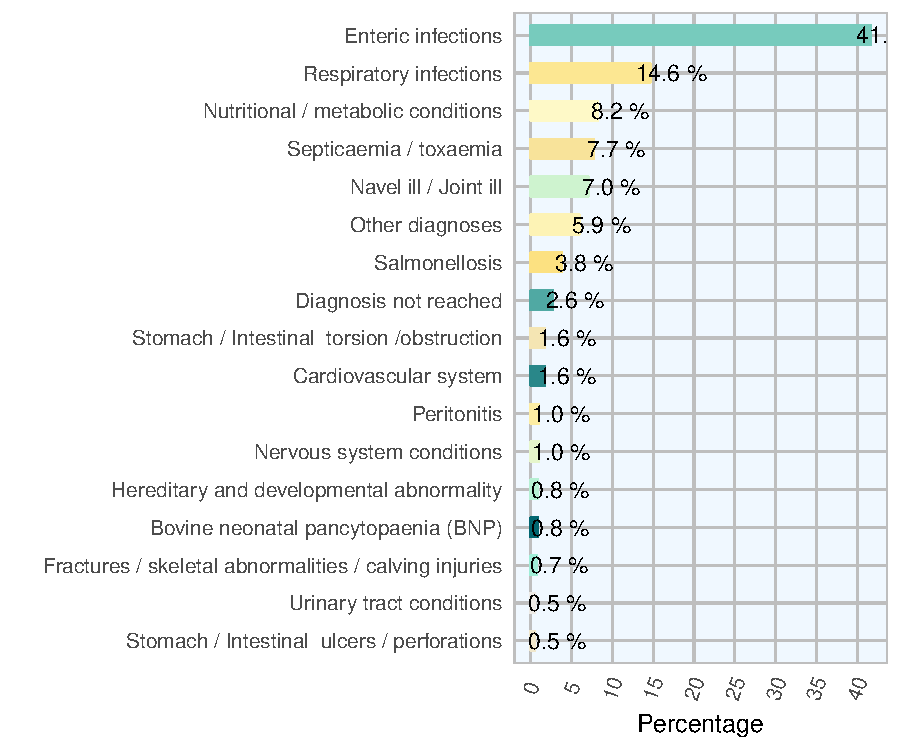
\includegraphics{AFBI_files/figure-latex/unnamed-chunk-7-1} 

}

\caption{The conditions most frequently diagnosed on post-mortem examinations of neonatal calves (0-1 months) by AFBI during 2017 (n= 610 )}\label{fig:unnamed-chunk-7}
\end{figure}

\section{Calves (1-5 months)}\label{calves-1-5-months}

Respiratory infections accounted for just over half of all deaths in
this age group in 2017 Northern Ireland, highlighting the economic and
welfare implications of respiratory disease (see the bovine respiratory
disease section below).

\begin{table}

\caption{\label{tab:unnamed-chunk-10}The conditions most frequently diagnosed on *post-mortem* examinations of calves (1-5 months) in  AFBI during 2017  (n= 369 )}
\centering
\begin{tabular}[t]{l|r|r}
\hline
Category & No. of cases & Percentage\\
\hline
Respiratory infections & 186 & 50.4\\
\hline
Enteric infections & 35 & 9.5\\
\hline
Diagnosis not reached & 19 & 5.2\\
\hline
Nutritional / metabolic conditions & 18 & 4.9\\
\hline
Stomach / Intestinal torsions /obstruction & 17 & 4.6\\
\hline
Peritonitis & 15 & 4.1\\
\hline
Other diagnoses & 14 & 3.8\\
\hline
Septicaemia / toxaemia & 13 & 3.5\\
\hline
Clostridial disease & 11 & 3.0\\
\hline
Navel ill / Joint ill & 11 & 3.0\\
\hline
Cardiovascular conditions & 9 & 2.4\\
\hline
Nervous system conditions & 6 & 1.6\\
\hline
Urinary tract conditions & 6 & 1.6\\
\hline
Stomach / Intestinal ulcer / perforation & 5 & 1.4\\
\hline
BVD / Mucosal disease & 2 & 0.5\\
\hline
Poisoning & 2 & 0.5\\
\hline
\end{tabular}
\end{table}

\begin{figure}

{\centering 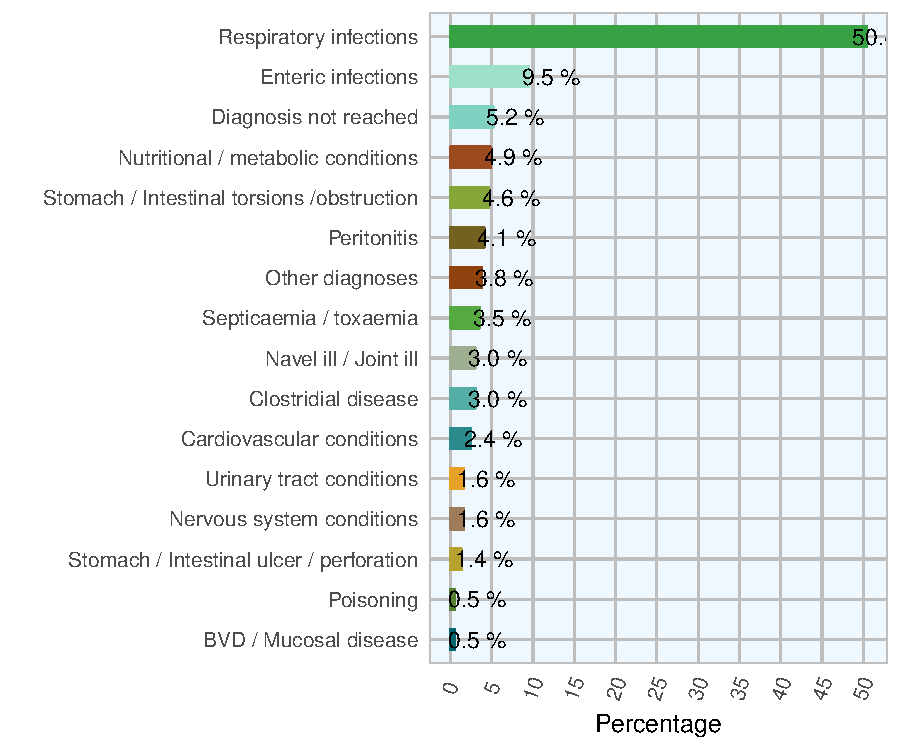
\includegraphics{AFBI_files/figure-latex/unnamed-chunk-11-1} 

}

\caption{The conditions most frequently diagnosed on *post-mortem* examinations of calves (1-5 months) by AFBI during 2017 (n= 369 )}\label{fig:unnamed-chunk-11}
\end{figure}

\begin{figure}

{\centering 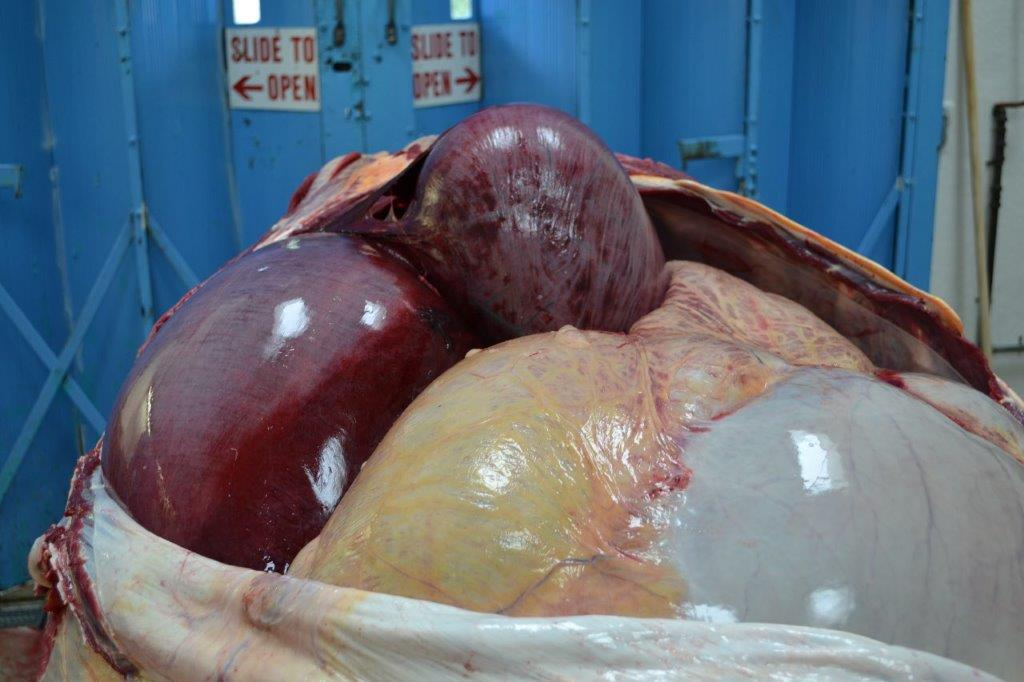
\includegraphics[width=14.22in]{_images/Torsion} 

}

\caption{Intestinal torsion. Photo:AFBI}\label{fig:torsion}
\end{figure}

\section{Calves (6-12 months)}\label{calves-6-12-months}

The most commonly diagnosed cause of death in this age group in 2017 was
respiratory infections which increased from 42\% of cases in 2016 to
49\% of cases in 2017. Clostridial diseases were identified as the
second largest cause of mortality in this age group in Northern Ireland
in 2017 despite the availability of cheap and efficacious vaccines.

\begin{table}

\caption{\label{tab:unnamed-chunk-13}The conditions most frequently diagnosed on *post-mortem* examinations of calves (6-12 months) in  AFBI during 2017 (n= 163 )}
\centering
\begin{tabular}[t]{l|r|r}
\hline
Category & No. of cases & Percentage\\
\hline
Respiratory tract infections & 80 & 49.1\\
\hline
Clostridial disease & 18 & 11.0\\
\hline
Diagnosis not reached & 17 & 10.4\\
\hline
Nutritional / metabolic conditions & 11 & 6.8\\
\hline
Enteric infections & 8 & 4.9\\
\hline
Other diagnoses & 6 & 3.7\\
\hline
Liver disease & 3 & 1.8\\
\hline
Poisoning & 3 & 1.8\\
\hline
Stomach / Intestinal ulcer, perforation, for body & 3 & 1.8\\
\hline
Urinary tract conditions & 3 & 1.8\\
\hline
BVD / Mucosal disease & 2 & 1.2\\
\hline
Cardiac conditions & 2 & 1.2\\
\hline
Nervous system conditions & 2 & 1.2\\
\hline
Skeletal conditions & 2 & 1.2\\
\hline
Stomach / Intestinal torsion / obstruction & 2 & 1.2\\
\hline
Peritonitis & 1 & 0.6\\
\hline
\end{tabular}
\end{table}

\begin{figure}

{\centering 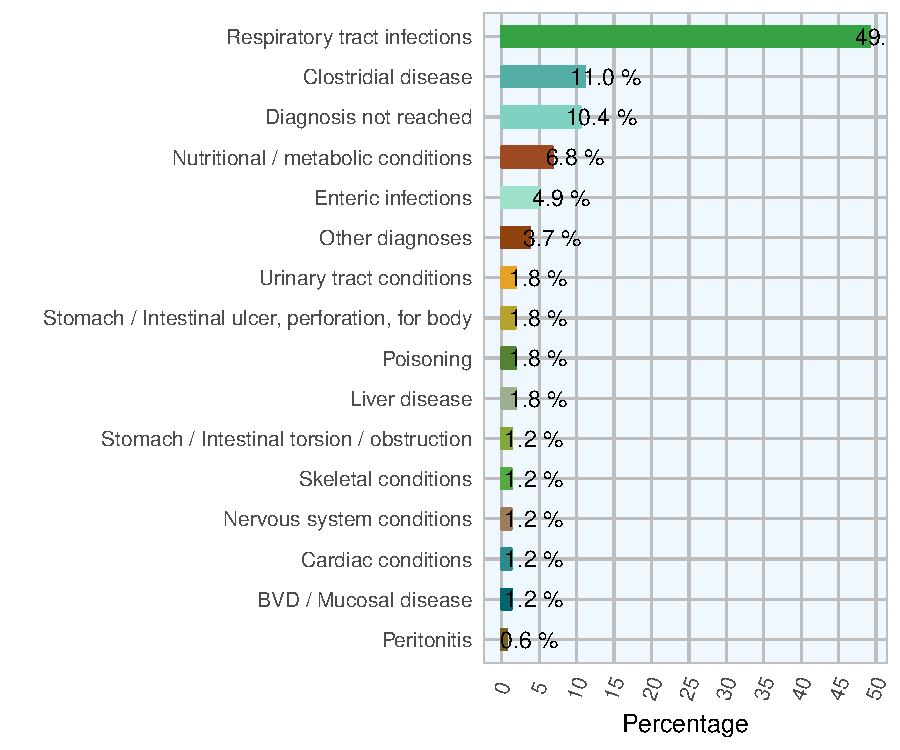
\includegraphics{AFBI_files/figure-latex/unnamed-chunk-14-1} 

}

\caption{The conditions most frequently diagnosed on *post-mortem* examinations of  calves (6-12 months) by AFBI during 2017 (n= 163 )}\label{fig:unnamed-chunk-14}
\end{figure}

\section{Adults (\textgreater{} 12 months)}\label{adults-12-months}

As in previous years, respiratory infections were identified as the most
common cause of death in adult cattle. Clostridial disease accounted for
8.4\% of adult cattle deaths in 2017, representing a decrease from the
10\% of cases in 2016. Cardiac/ circulatory system conditions such as
endocarditis, pericarditis and caudal vena cava thrombosis were also a
common cause of mortality in adult cows in 2017.

\begin{table}

\caption{\label{tab:unnamed-chunk-16}The conditions most frequently diagnosed on *post-mortem* examinations of adults (>12 months) by AFBI during 2017 (n= 464 )}
\centering
\begin{tabular}[t]{l|r|r}
\hline
Category & No. of cases & Percentage\\
\hline
Respiratory infections & 95 & 20.5\\
\hline
Other diagnoses & 56 & 12.1\\
\hline
Diagnosis not reached & 55 & 11.8\\
\hline
Cardiac / circulatory system & 50 & 10.8\\
\hline
Clostridial disease & 39 & 8.4\\
\hline
Nutritional / metabolic conditions & 36 & 7.8\\
\hline
Liver disease & 29 & 6.2\\
\hline
Stomach / Intestinal ulceration / perforation / foreign body & 24 & 5.2\\
\hline
Enteric infections & 19 & 4.1\\
\hline
Reproductive tract infections / Mastitis & 12 & 2.6\\
\hline
Intestinal or gastric torsion / obstruction & 10 & 2.2\\
\hline
Peritonitis & 10 & 2.2\\
\hline
Poisoning & 9 & 1.9\\
\hline
Urinary tract conditions & 9 & 1.9\\
\hline
Tumour & 6 & 1.3\\
\hline
Nervous system conditions & 5 & 1.1\\
\hline
\end{tabular}
\end{table}

\begin{figure}

{\centering 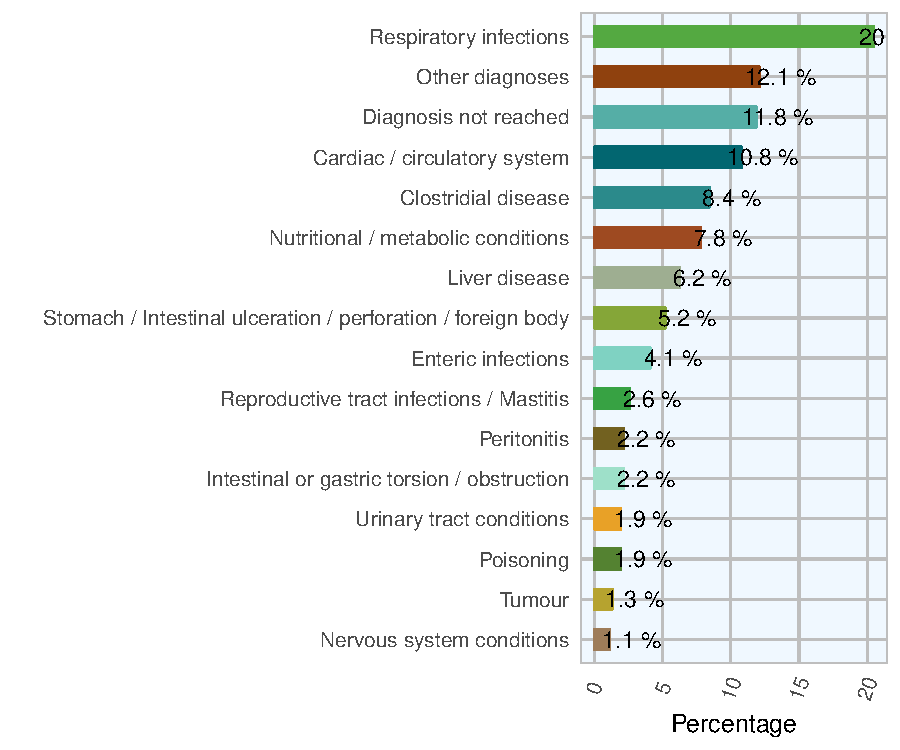
\includegraphics{AFBI_files/figure-latex/unnamed-chunk-17-1} 

}

\caption{The conditions most frequently diagnosed on *post-mortem* examinations of  adults (>12 months) by AFBI during 2017, (n= 464 )}\label{fig:unnamed-chunk-17}
\end{figure}

\chapter{Bovine Respiratory Disease
(BRD)}\label{bovine-respiratory-disease-brd}

\begin{center}\rule{0.5\linewidth}{\linethickness}\end{center}

Bovine respiratory disease was the most commonly identified cause of
death in all age groups of bovines, other than neonatal calves,
submitted to AFBI in 2017 and was the second most commonly identified
cause of death in neonatal calves. There were multiple aetiologies for
respiratory infections identified. As in 2016 \emph{Mycoplasma bovis}
was the pathogen identified with the greatest frequency from cattle
diagnosed with respiratory disease in 2017. At AFBI \emph{Mycoplasma
bovis} is detected by a PCR testing and positive results need to be
interpreted in conjunction with gross and histopathological findings.
Environmental factors also play a role in the condition. Parasitic
bronchitis due to the lungworm \emph{Dictyocaulus viviparus} (Figure
\ref{fig:foo3}) was seen in 6.9\% of bovine respiratory disease
diagnoses cases with the expected seasonal peak in August. The economic
cost of wastage and reduced productivity due to respiratory infections
in the cattle industry is considerable.

\section{Diagnoses by Group}\label{diagnoses-by-group}

\begin{table}

\caption{\label{tab:unnamed-chunk-21}The most common diagnostic groups on *post-mortem* examinations of bovine respiratory disease by AFBI during 2017 (n= 391 )}
\centering
\begin{tabular}[t]{l|r|r}
\hline
Category & No. of cases & Percentage\\
\hline
Bacterial & 220 & 56.3\\
\hline
Other & 135 & 34.5\\
\hline
Viral & 36 & 9.2\\
\hline
\end{tabular}
\end{table}

\begin{figure}

{\centering 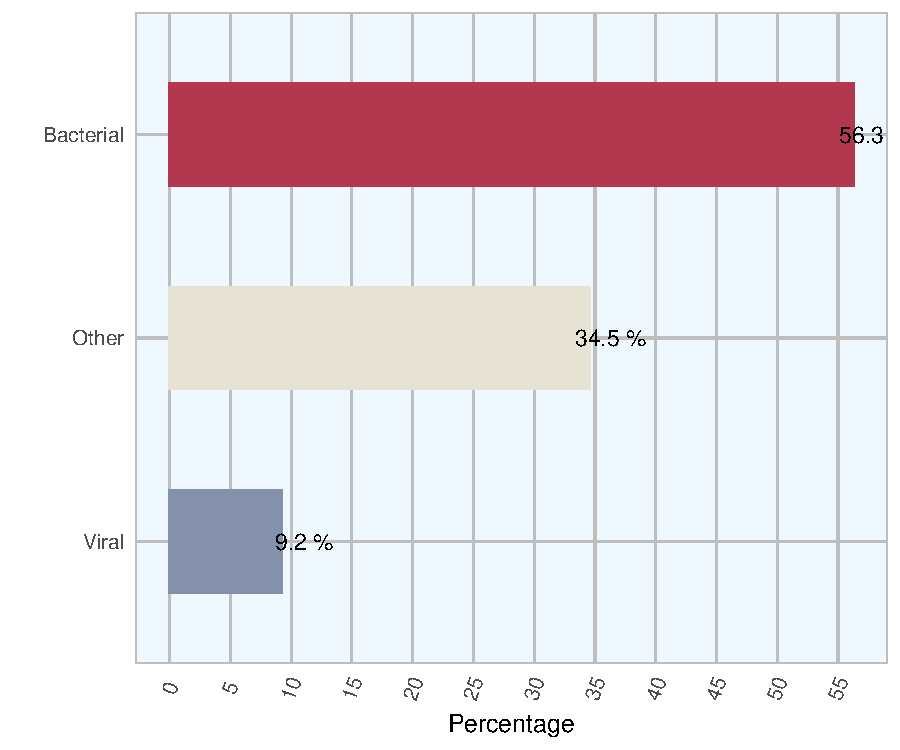
\includegraphics{AFBI_files/figure-latex/unnamed-chunk-22-1} 

}

\caption{The most common diagnostic groups on *post-mortem* examinations of bovine respiratory disease by AFBI during 2017 (n= 391 )}\label{fig:unnamed-chunk-22}
\end{figure}

\subsection{Bovine Respiratory Disease
Diagnoses}\label{bovine-respiratory-disease-diagnoses}

\begin{table}

\caption{\label{tab:unnamed-chunk-26}Relative frequency of diagnoses in bovine respiratory disease recorded by AFBI during 2017, (n= 388 )}
\centering
\begin{tabular}[t]{l|r|r}
\hline
Category & No. of cases & Percentage\\
\hline
PNEUMONIA DT MYCOPLASMA BOVIS & 90 & 23.2\\
\hline
PNEUMONIA NOS & 70 & 18.0\\
\hline
PNEUMONIA DT P MULTOCIDA & 45 & 11.6\\
\hline
PNEUMONIA A PYOGENES & 35 & 9.0\\
\hline
PNEUMONIA DT M HAEMOLYTICA & 33 & 8.5\\
\hline
PNEUMONIA - PARASITIC - HUSK & 27 & 7.0\\
\hline
PNEUMONIA - RSV & 15 & 3.9\\
\hline
FIBRINOUS PLEURISY & 14 & 3.6\\
\hline
IBR & 12 & 3.1\\
\hline
PNEUMONIA - H SOMNUS & 10 & 2.6\\
\hline
CHRONIC BRONCHOPNEUMONIA & 6 & 1.6\\
\hline
PNEUMONIA - BVD & 5 & 1.3\\
\hline
PNEUMONIA DT ASPIRATION & 4 & 1.0\\
\hline
SEVERE TRACHEITIS & 4 & 1.0\\
\hline
PASTEURELLOSIS & 3 & 0.8\\
\hline
MALIGNANT CATARRH & 2 & 0.5\\
\hline
PNEUMONIA - FUNGAL & 2 & 0.5\\
\hline
PNEUMONIA - P13 & 2 & 0.5\\
\hline
PNEUMONIA DT ACTINO & 2 & 0.5\\
\hline
PULMONARY EMBOLISM & 2 & 0.5\\
\hline
TUBERCULOSIS & 2 & 0.5\\
\hline
ADENOCARCINOMA & 1 & 0.3\\
\hline
ATELECTASIS & 1 & 0.3\\
\hline
PULMONARYHAEMORRHAGE & 1 & 0.3\\
\hline
\end{tabular}
\end{table}

\begin{figure}

{\centering 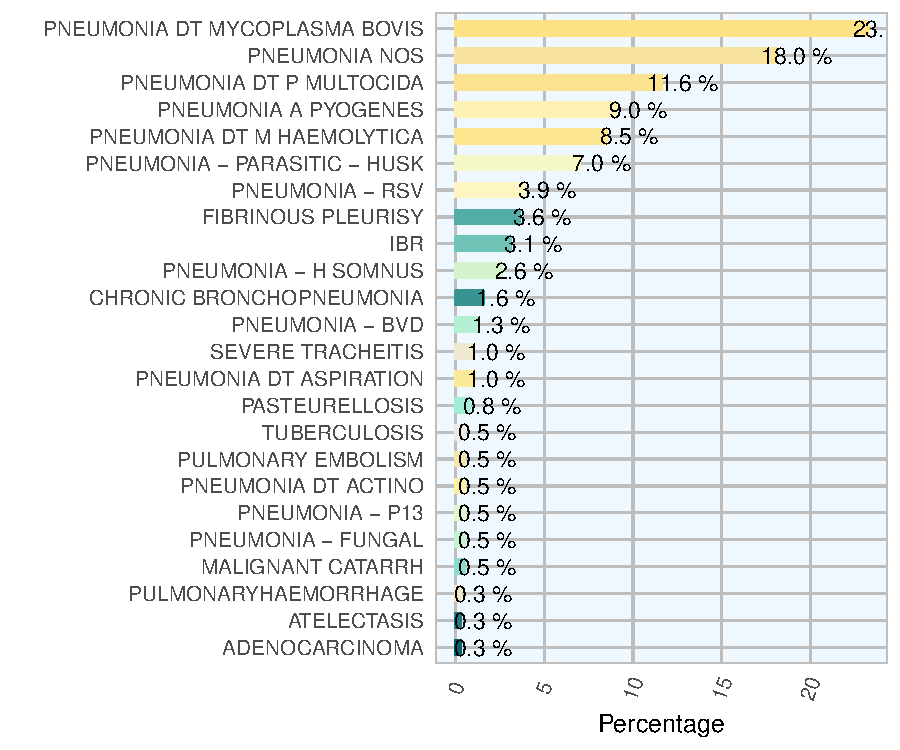
\includegraphics{AFBI_files/figure-latex/unnamed-chunk-27-1} 

}

\caption{Relative frequency of diagnoses in bovine respiratory disease recorded by AFBI during 2017, (n= 388 )}\label{fig:unnamed-chunk-27}
\end{figure}

\subsection{Lungworm}\label{lungworm}

\begin{figure}

{\centering 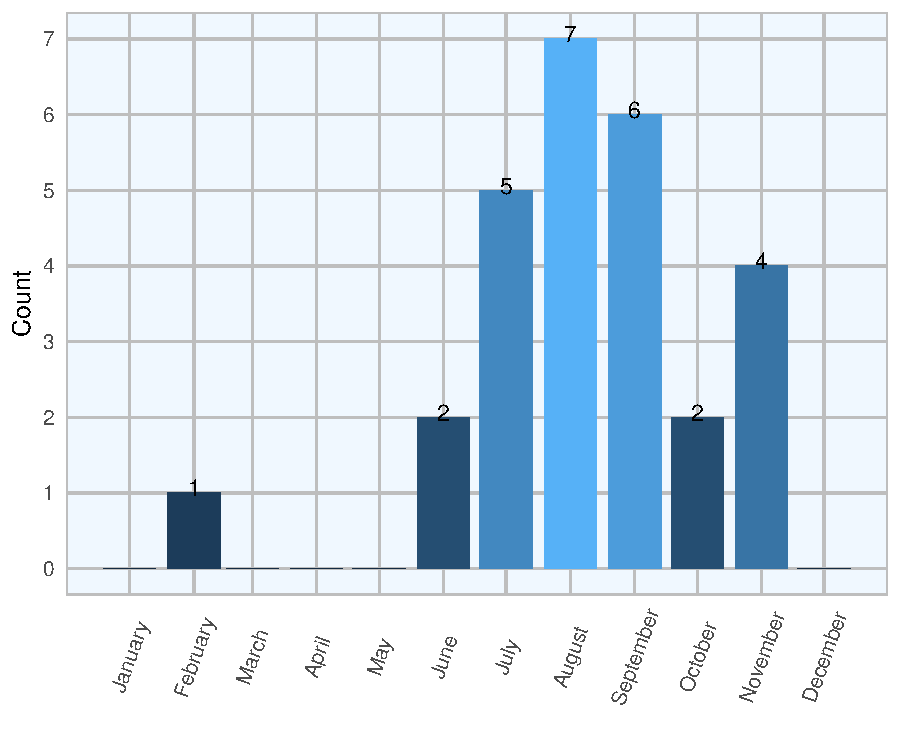
\includegraphics{AFBI_files/figure-latex/unnamed-chunk-30-1} 

}

\caption{Cases of death due to lungworm in cattle recorded by AFBI during 2017, (n= 27 )}\label{fig:unnamed-chunk-30}
\end{figure}

\begin{figure}

{\centering 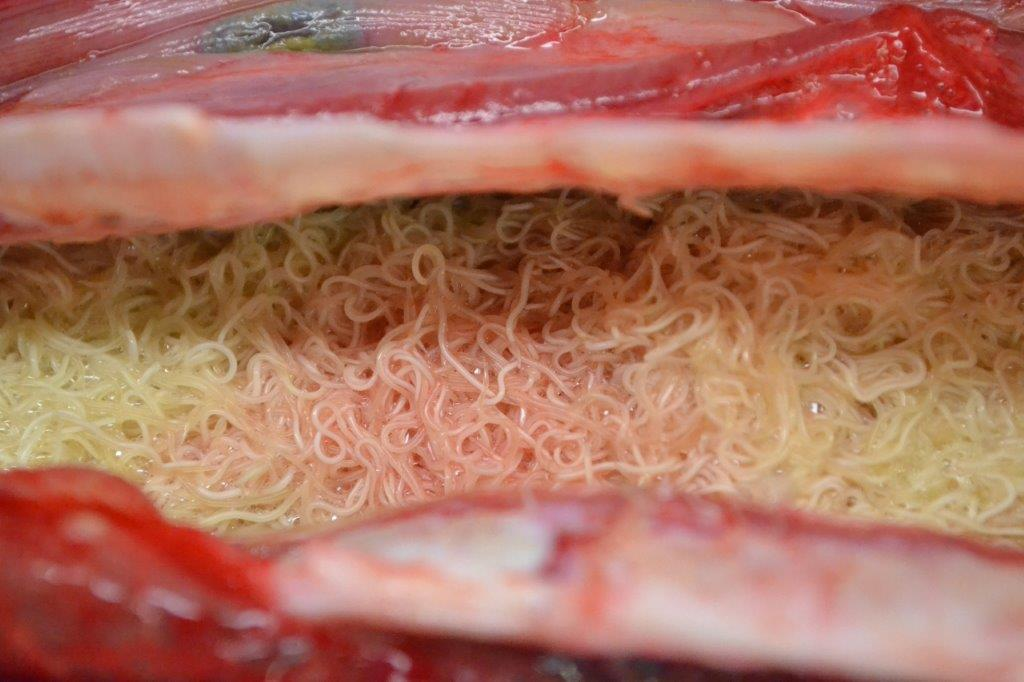
\includegraphics[width=14.22in]{_images/Lungworm} 

}

\caption{Trachea containing large numbers of lungworm (*Dictyocaulus viviparus*). Photo:AFBI}\label{fig:foo3}
\end{figure}

\chapter{Bovine Abortions}\label{bovine-abortions}

\begin{center}\rule{0.5\linewidth}{\linethickness}\end{center}

Bovine abortion is a significant cause of livestock wastage and results
in considerable costs to the cattle industry. As a general guideline
once the level of abortions exceeds 3\% or if there are several
abortions clustered together investigation should be carried out.
Specimens from 427 bovine abortions and stillbirths were examined during
2017 (430 were examined in 2016). Significant pathogens were detected in
198 of these (46\%). This diagnostic rate is comparable to other years
and reflects the multiple aetiologies of bovine abortion and the fact
that not all abortions are due to an infectious cause. \emph{Trueperella
pyogenes} and \emph{Bacillus licheniformis} were the most commonly
diagnosed pathogens as in previous years. \emph{Neospora caninum} was
the third most commonly diagnosed pathogen followed by \emph{Salmonella
Dublin} BVDV and \emph{E.coli}. \emph{T. pyogenes} is considered a
sporadic cause of abortion through haematogenous spread and placentitis.
\emph{Bacillus licheniformis} also results in placentitis. \emph{B.
licheniformis} is ubiquitous, although silage, run-off water, foodstuffs
and bedding that have become contaminated with silage effluent and wet
spoiled hay are the most likely sources of infection.

\begin{table}

\caption{\label{tab:unnamed-chunk-34}The most frequently diagnosed causes of cattle abortion diagnosed at AFBI in 2017 (n= 427 )}
\centering
\begin{tabular}[t]{l|r|r}
\hline
Category & Count & Percentage\\
\hline
Diagnosis not reached & 229 & 53.6\\
\hline
T. pyogenes & 37 & 8.7\\
\hline
B. licheniformis & 35 & 8.2\\
\hline
N. caninum & 21 & 4.9\\
\hline
Other & 17 & 4.0\\
\hline
BVDV & 15 & 3.5\\
\hline
E. coli & 15 & 3.5\\
\hline
S. Dublin & 15 & 3.5\\
\hline
Leptospirosis & 12 & 2.8\\
\hline
Pasteurellosis & 9 & 2.1\\
\hline
Foetal abnormalities & 8 & 1.9\\
\hline
Schmallenberg Virus & 5 & 1.2\\
\hline
Listeria & 4 & 0.9\\
\hline
Campylobacter sp & 3 & 0.7\\
\hline
Aspergillosis & 2 & 0.5\\
\hline
\end{tabular}
\end{table}

\begin{figure}

{\centering 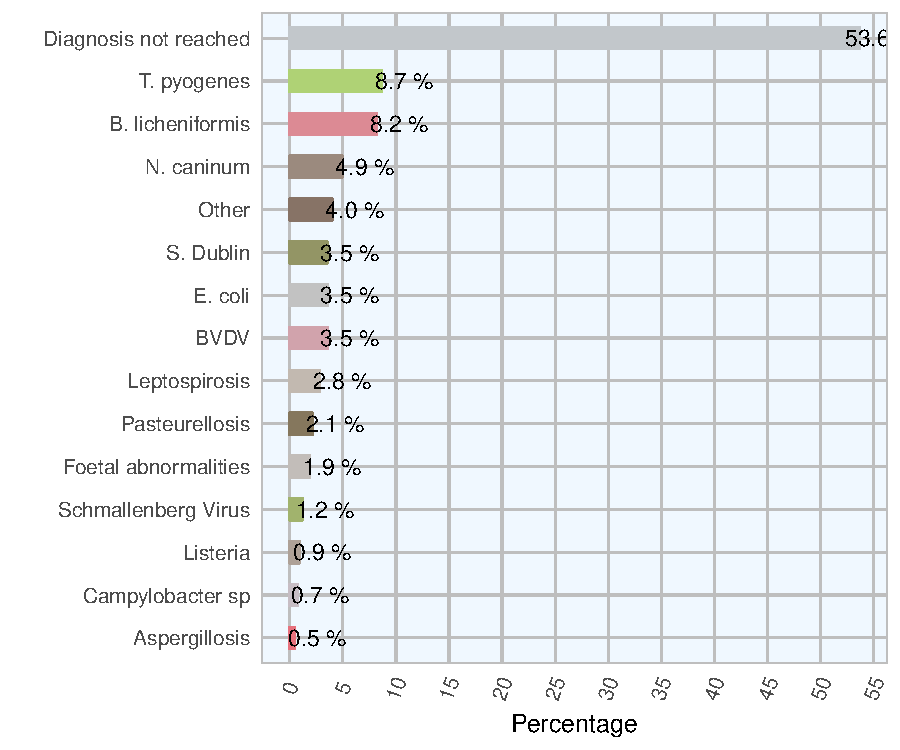
\includegraphics{AFBI_files/figure-latex/unnamed-chunk-35-1} 

}

\caption{The most frequently diagnosed causes of cattle abortion diagnosed at AFBI in 2017 (n= 427 )}\label{fig:unnamed-chunk-35}
\end{figure}

\section{Salmonella Dublin Abortion}\label{salmonella-dublin-abortion}

\begin{figure}

{\centering 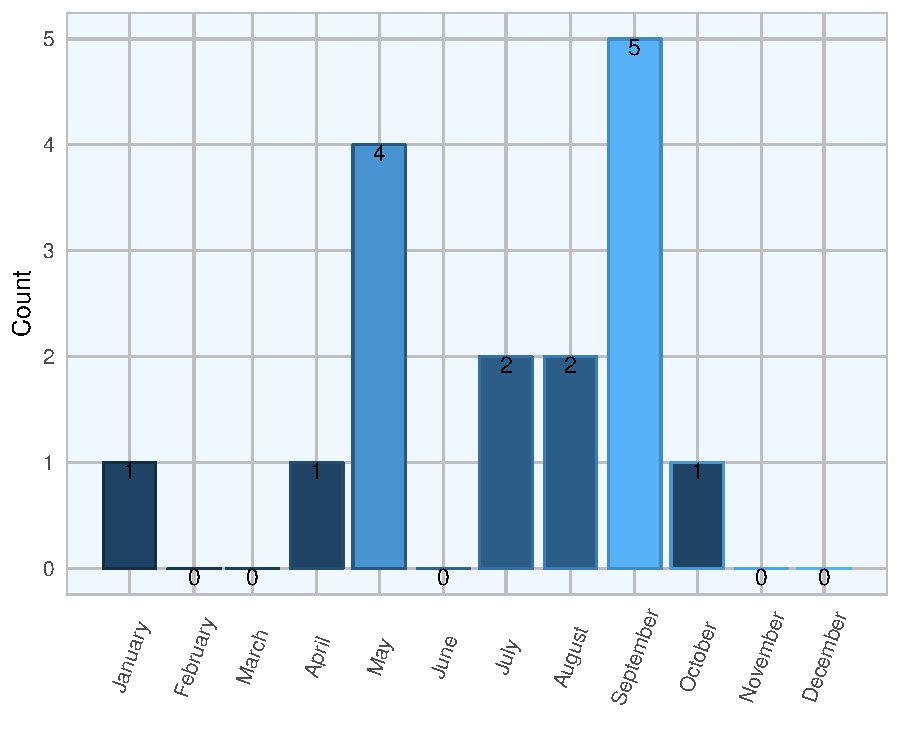
\includegraphics{AFBI_files/figure-latex/salm1-1} 

}

\caption{Diagnosis of abortion due to *Salmonella Dublin* in 2017}\label{fig:salm1}
\end{figure}

\chapter{Clostridial Diseases}\label{clostridial-diseases}

\begin{center}\rule{0.5\linewidth}{\linethickness}\end{center}

\begin{table}

\caption{\label{tab:unnamed-chunk-40}Clostridial Diseases}
\centering
\begin{tabular}[t]{l|r}
\hline
Clostridial disease & Number of Cases\\
\hline
Blackleg & 31\\
\hline
Botulism & 12\\
\hline
Black disease & 11\\
\hline
Clostridium perfringens & 1\\
\hline
Malignant oedema & 1\\
\hline
\end{tabular}
\end{table}

\begin{figure}

{\centering 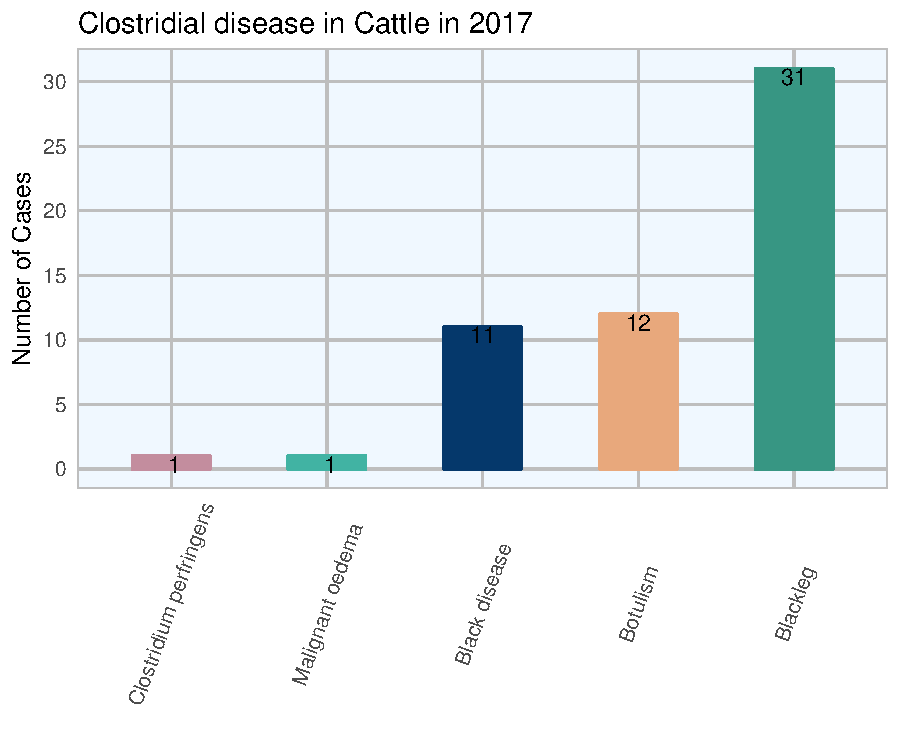
\includegraphics{AFBI_files/figure-latex/unnamed-chunk-41-1} 

}

\caption{Clostridial disease in Cattle in 2017}\label{fig:unnamed-chunk-41}
\end{figure}

\begin{figure}

{\centering 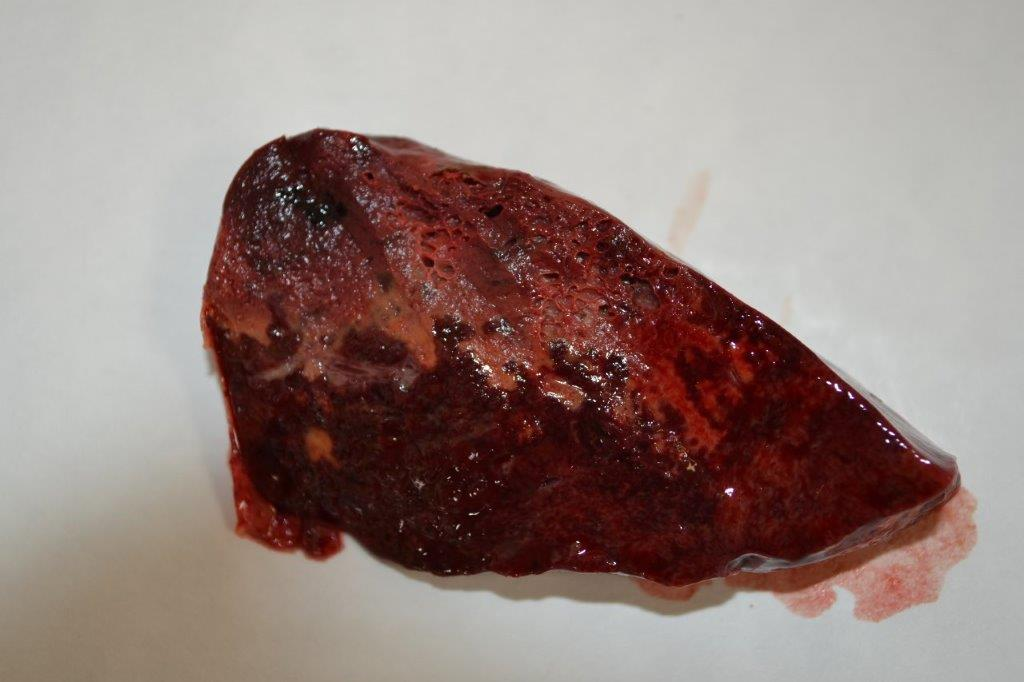
\includegraphics[width=14.22in]{_images/blackDisease} 

}

\caption{: Pale focus typical of black disease in a bovine liver. Photo:AFBI}\label{fig:foo2}
\end{figure}

\begin{center}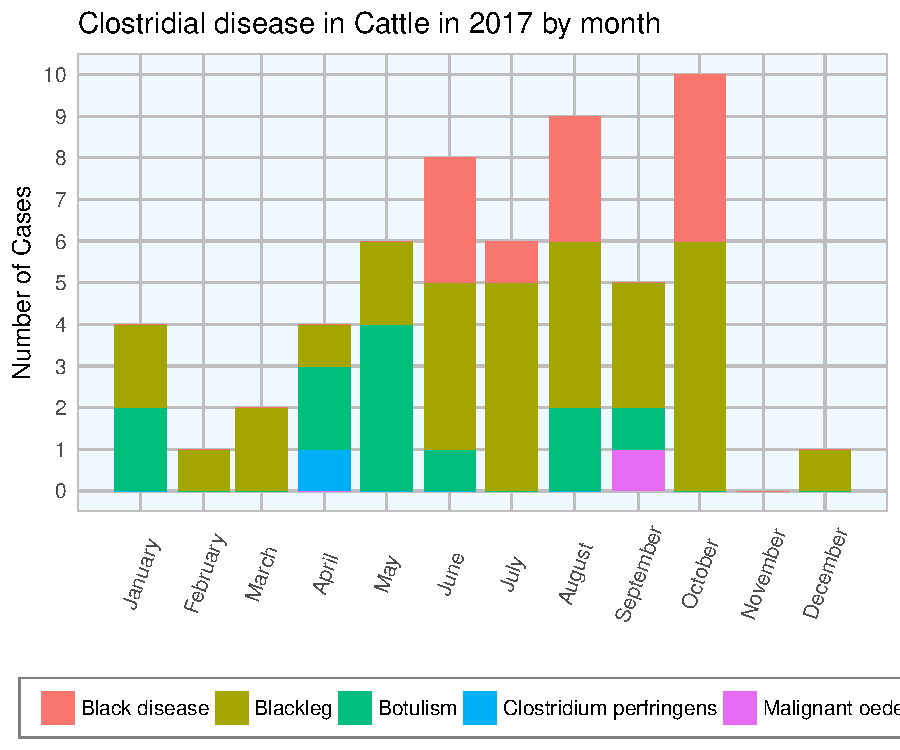
\includegraphics{AFBI_files/figure-latex/unnamed-chunk-42-1} \end{center}

\begin{figure}

{\centering 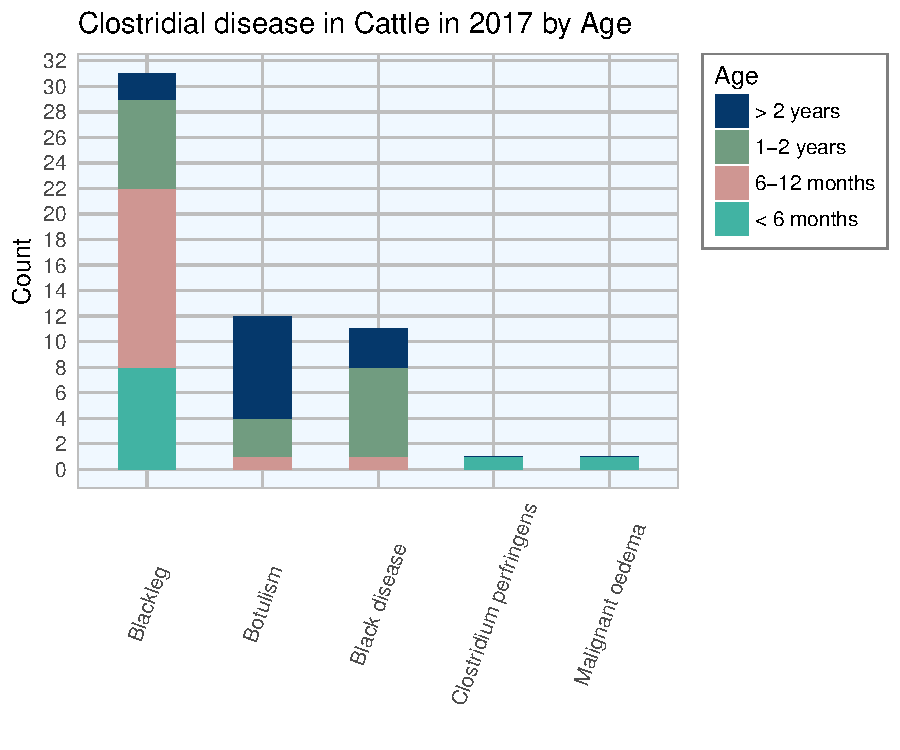
\includegraphics{AFBI_files/figure-latex/unnamed-chunk-44-1} 

}

\caption{Clostridial disease in Cattle in 2017}\label{fig:unnamed-chunk-44}
\end{figure}

\chapter{Bovine Mastitis}\label{bovine-mastitis}

\begin{center}\rule{0.5\linewidth}{\linethickness}\end{center}

A total of 1147 bacterial isolates were cultured from milk samples
submitted from acute and chronic mastitis cases. Significance of the
organism depends on the cell count, the level of the organism isolated
and whether or not the organism was isolated in pure culture. Isolation
of 3 or more species suggests contamination during sampling.
Interpretation of the results should therefore be undertaken with care.
Submission of contaminated samples has dropped from 10.6\% of samples in
2016 to 9.6\% in 2017. E.coli was the most frequently isolated organism
accounting for 22.8\% of isolates cultured (compared with 23.7\% in
2016). \emph{E.coli} is the most prevalent environmental cause of
mastitis. Risk factors include poor hygiene, suboptimal milking machine
function, teat end damage and lactation. Another frequently identified
environmental organism, \emph{Streptococcus uberis} was identified in
13.6\% of submitted samples,a decline on previous years.
\emph{Staphylococcus aureus}, a ``contagious'' cause of mastitis,
typically spread from cow to cow via the milking equipment was
identified in 8.5\% of samples submitted in 2017, compared to 8.1\% in
2016.

\begin{table}

\caption{\label{tab:unnamed-chunk-48}Bacteria isolated on culture of milk samples submitted to AFBI in 2017}
\centering
\begin{tabular}[t]{l|r|r}
\hline
Microorganism & No. of cases & Percentage\\
\hline
E.coli & 261 & 22.8\\
\hline
Streptococcus uberis & 156 & 13.6\\
\hline
Staphlococcus aureus & 97 & 8.5\\
\hline
Streptococcus dysgalactiae & 28 & 2.4\\
\hline
Contaminated samples & 110 & 9.6\\
\hline
No bacteria cultured & 143 & 12.5\\
\hline
Other & 352 & 30.7\\
\hline
\end{tabular}
\end{table}

\begin{figure}

{\centering 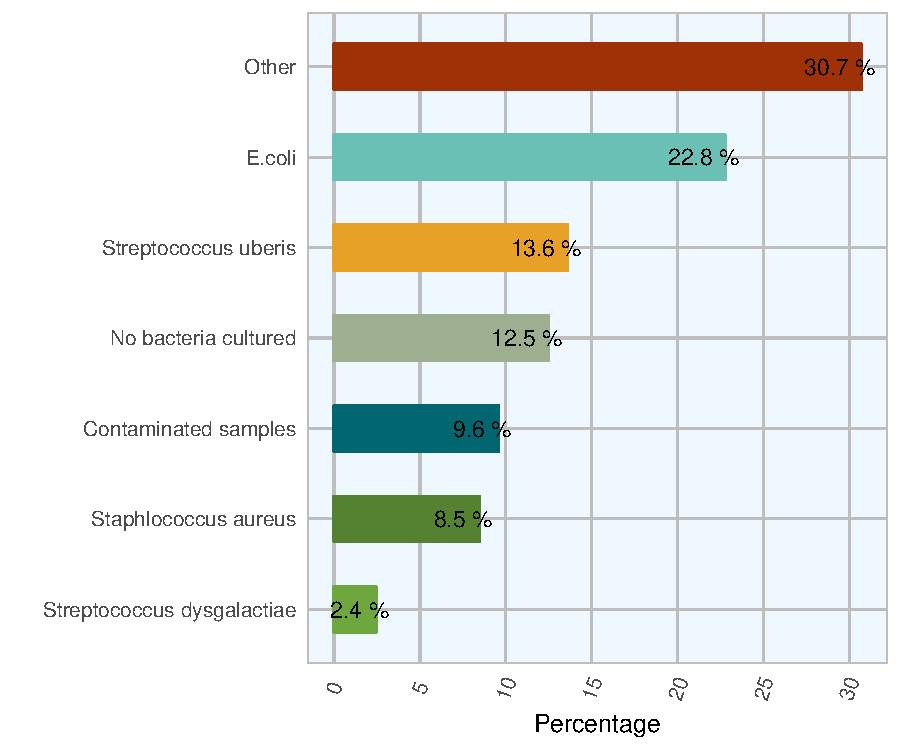
\includegraphics{AFBI_files/figure-latex/unnamed-chunk-49-1} 

}

\caption{Bacteria isolated on culture of milk samples submitted to AFBI in 2017}\label{fig:unnamed-chunk-49}
\end{figure}

\chapter{Bovine Parasites}\label{bovine-parasites}

\begin{center}\rule{0.5\linewidth}{\linethickness}\end{center}

\section{Trichostrongyle eggs}\label{trichostrongyle-eggs}

\begin{figure}

{\centering 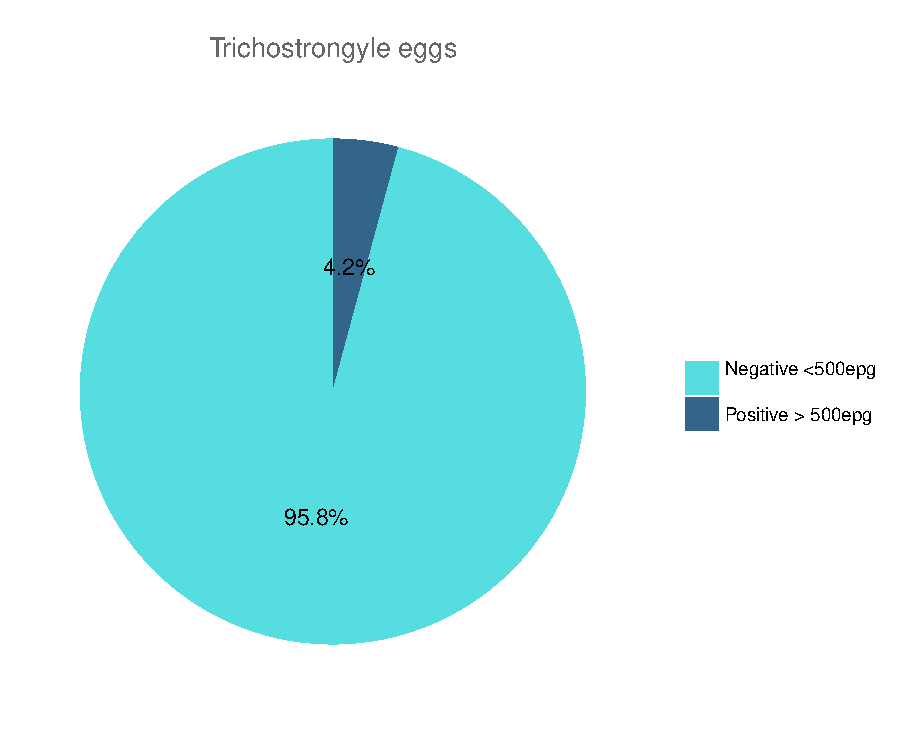
\includegraphics{AFBI_files/figure-latex/unnamed-chunk-53-1} 

}

\caption{Relative frequency of detection of trichostrongyle eggs in bovine faecal samples examined in AFBI in 2017 in relation to a commonly used threshold of significance- 500 eggs per gram (n=3008)}\label{fig:unnamed-chunk-53}
\end{figure}

\section{Liver fluke eggs}\label{liver-fluke-eggs}

\begin{figure}

{\centering 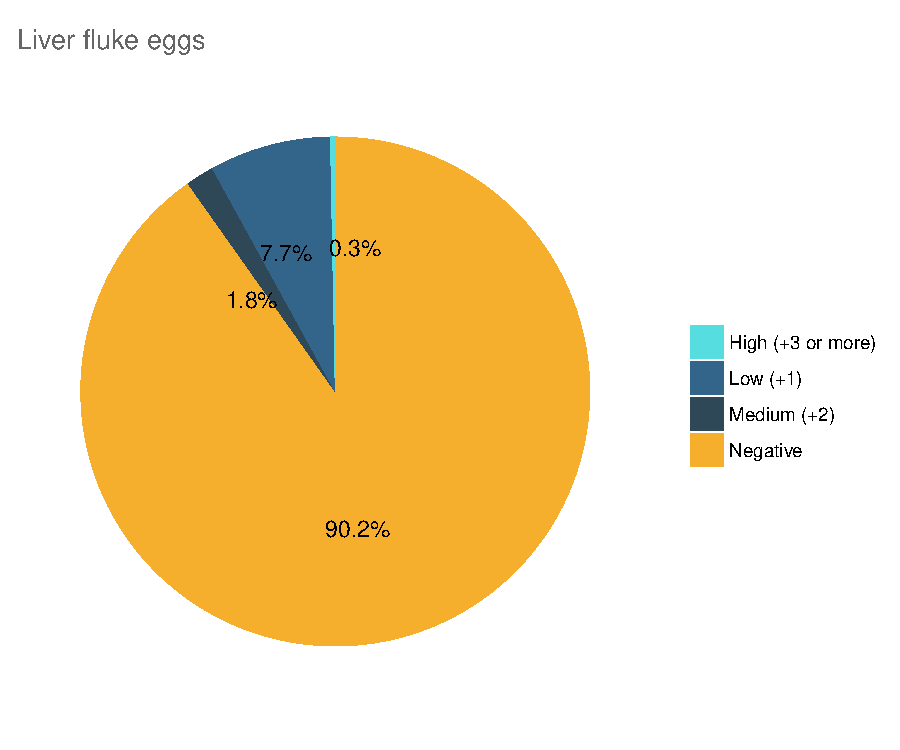
\includegraphics{AFBI_files/figure-latex/unnamed-chunk-55-1} 

}

\caption{AFBI results for bovine faecal samples tested for liver fluke eggs during 2017 (n=2751)}\label{fig:unnamed-chunk-55}
\end{figure}

\section{Rumen fluke eggs}\label{rumen-fluke-eggs}

\begin{figure}

{\centering 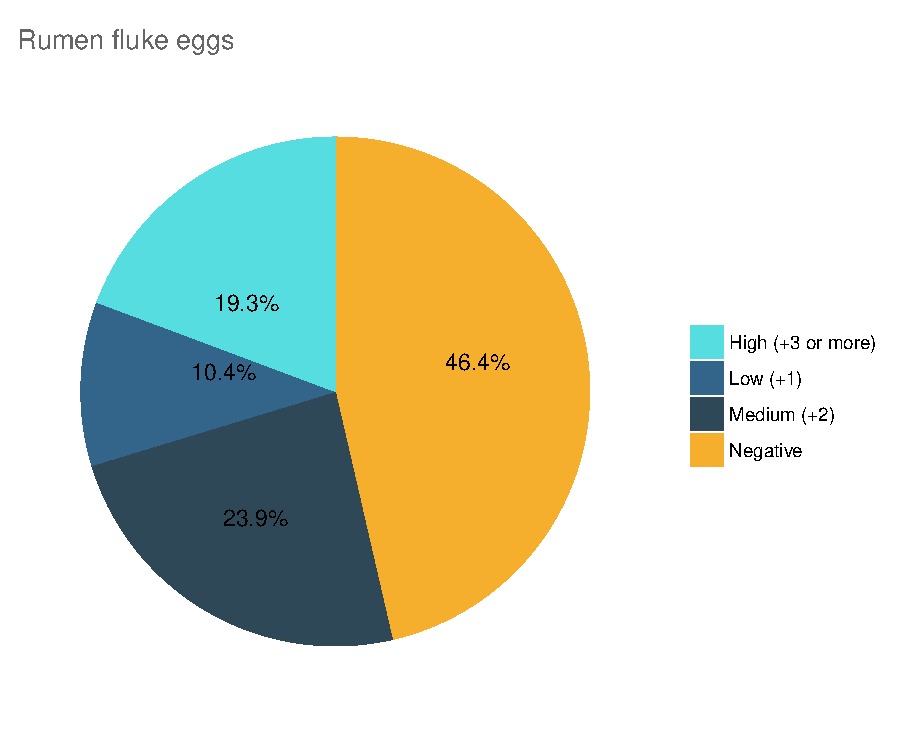
\includegraphics{AFBI_files/figure-latex/unnamed-chunk-57-1} 

}

\caption{AFBI results for bovine faecal samples tested for paramphistome eggs during 2017 (n=2730)}\label{fig:unnamed-chunk-57}
\end{figure}

\section{Coccidia}\label{coccidia}

\begin{figure}

{\centering 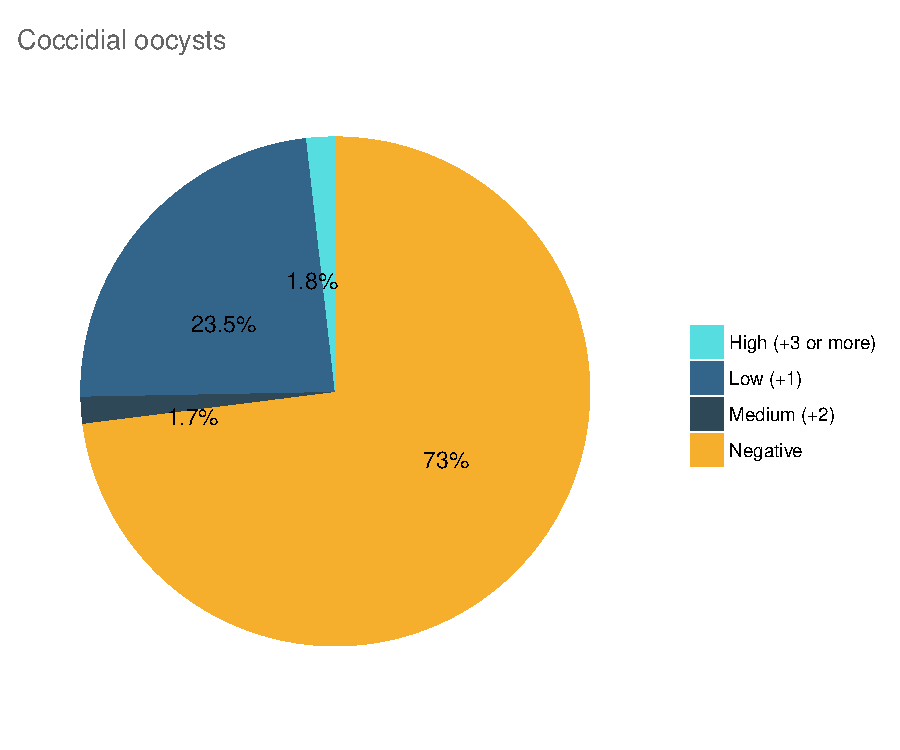
\includegraphics{AFBI_files/figure-latex/unnamed-chunk-59-1} 

}

\caption{AFBI results for bovine faecal samples tested for coccidial oocysts during 2017 (n=3019)}\label{fig:unnamed-chunk-59}
\end{figure}

\chapter{Bovine Neonatal Enteritis}\label{bovine-neonatal-enteritis}

\begin{center}\rule{0.5\linewidth}{\linethickness}\end{center}

863 neonatal faecal samples were examined by AFBI in 2017. As in
previous years Cryptosporidium was the most regularly identified
pathogen, identified in 37\% of cases, rotavirus was the second most
regularly identified pathogen, identified in 30\% of cases and
coronavirus was identified in 11\% of cases. Faecal samples sent to AFBI
from calves less than two weeks of age are also checked for the presence
of \emph{E.coli} expressing the K99 fimbrial antigen. \emph{E.coli} K99
has been associated with enterotoxigenic colibacillosis in neonates. In
2017 \emph{E.coli} K99 was identified in 3\% of faecal samples from
calves less than 2 weeks of age.

\begin{table}

\caption{\label{tab:unnamed-chunk-67}Bovine Neonatal Enteritis}
\centering
\begin{tabular}[t]{l|r|r|r}
\hline
Organism & Tested & Positive & Percentage of samples tested\\
\hline
Cryptosporidium & 863 & 320 & 37.1\\
\hline
Rotavirus & 860 & 259 & 30.1\\
\hline
Coronavirus & 863 & 94 & 10.9\\
\hline
E.coli K99 & 494 & 15 & 3.0\\
\hline
Salmonella & 863 & 31 & 3.6\\
\hline
\end{tabular}
\end{table}

\begin{figure}

{\centering 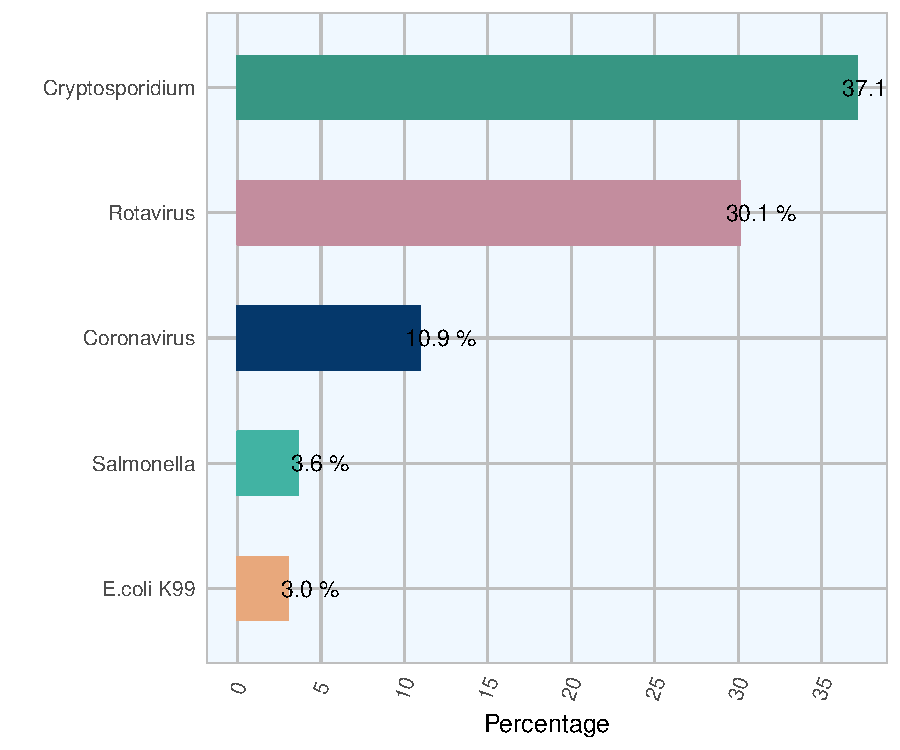
\includegraphics{AFBI_files/figure-latex/unnamed-chunk-68-1} 

}

\caption{Bovine Neonatal Enteritis}\label{fig:unnamed-chunk-68}
\end{figure}

\chapter{Zinc Sulphate Turbidity (ZST)
Test}\label{zinc-sulphate-turbidity-zst-test}

\begin{center}\rule{0.5\linewidth}{\linethickness}\end{center}

The Zinc Sulphate Turbidity test is an indirect measurement of the
passive transfer of immunoglobulins from the dam to the neonate. During
2017, 864 blood samples (submitted by veterinary practitioners or
collected at post-mortem examination of carcases at AFBI) were tested by
AFBI and of these 465 (54\%) returned a value of less than 20 units
i.e.~there had been inadequate passive transfer of immunoglobulins in
this individual. Further analysis shows that of the 648 blood samples
submitted by vets in practice, 324 (50\%) were inadequate and of the 216
samples taken during a post mortem 141 (65\%) were inadequate, this
highlights the link between calf mortality and inadequate passive
transfer of immunoglobulins.

\begin{table}

\caption{\label{tab:unnamed-chunk-72}Zinc Sulphate Turbidity Test}
\centering
\begin{tabular}[t]{l|r|r|r|r|r}
\hline
Status & Count & Mean & Median & Minimum & Maximum\\
\hline
Adequate & 407 & 30 & 27 & 0 & 111\\
\hline
Low & 457 & 11 & 11 & 1 & 19\\
\hline
\end{tabular}
\end{table}

\chapter{Ovine Diseases}\label{ovine-diseases}

\begin{center}\rule{0.5\linewidth}{\linethickness}\end{center}

The number of sheep submissions in Northern Ireland decreased slightly
in 2017 compared to 2016 perhaps reflecting the economic situation of
the sheep sector during the year and also the higher levels of parasitic
disease seen in the autumn and early winter of 2016.

As in 2016, parasitic disease and respiratory disease were the most
commonly diagnosed causes of death in sheep of all ages in Northern
Ireland. The relative importance of clostridial diseases increased
slightly in 2017 compared to 2016.

\begin{table}

\caption{\label{tab:unnamed-chunk-78}Conditions most frequently diagnosed on *post-mortem* examination of sheep by AFBI in 2017 (n= 559 )}
\centering
\begin{tabular}[t]{l|r|r}
\hline
Category & No. of cases & Percentage\\
\hline
Parasitic Disease & 188 & 33.6\\
\hline
Enteritis & 158 & 28.3\\
\hline
Respiratory Disease & 73 & 13.1\\
\hline
Septicaemia & 36 & 6.4\\
\hline
Clostridial diseases & 32 & 5.7\\
\hline
Nervous system conditions & 27 & 4.8\\
\hline
Metabolic conditions & 23 & 4.1\\
\hline
Poisoning & 22 & 3.9\\
\hline
\end{tabular}
\end{table}

\begin{figure}

{\centering 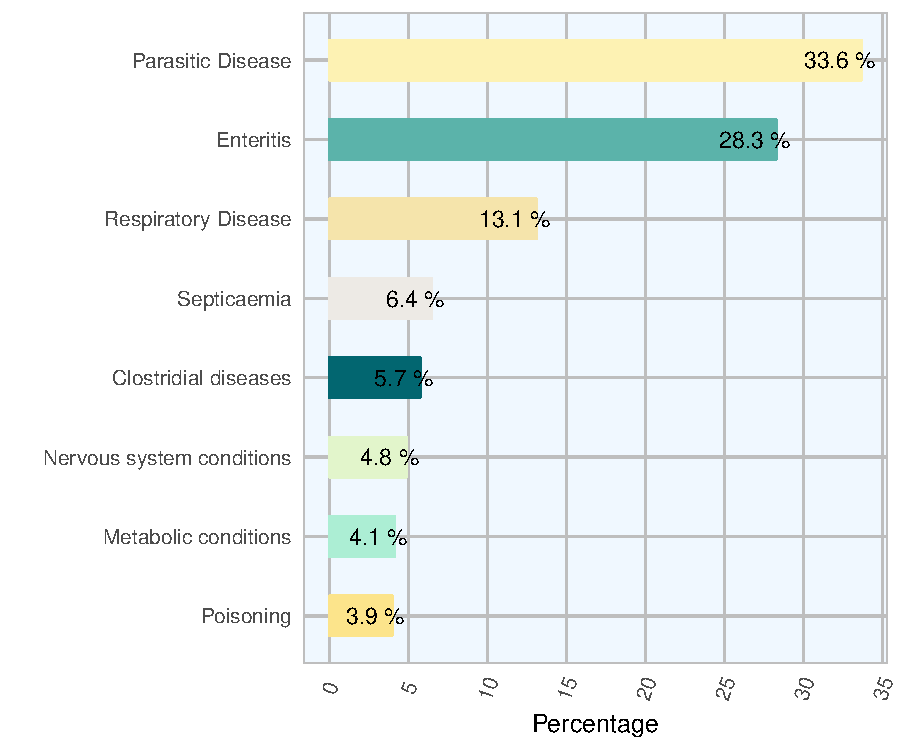
\includegraphics{AFBI_files/figure-latex/unnamed-chunk-79-1} 

}

\caption{The conditions most frequently diagnosed on *post-mortem* examinations of  ovine carcases in 2017(n= 559 )}\label{fig:unnamed-chunk-79}
\end{figure}

\section{Causes of sheep mortality in
2017}\label{causes-of-sheep-mortality-in-2017}

\subsection{Septicaemia}\label{septicaemia}

Pasteurellosis was the most frequently diagnosed septicaemic cause of
mortality in sheep in 2017 despite the availability of protective
vaccines against pasteurellosis. Careful vaccination of breeding stock
and if necessary finishing lambs is an effective way of reducing
pasteurellosis.

\begin{table}

\caption{\label{tab:unnamed-chunk-83}The relative frequency of diagnoses of septicaemic conditions on *post-mortem* examination of sheep in 2017 (n= 36 )}
\centering
\begin{tabular}[t]{l|r|r}
\hline
Disease & No. of cases & Percentage of total diagnoses\\
\hline
Pasteurella septicaemia & 18 & 3.2\\
\hline
Colisepticaemia & 9 & 1.6\\
\hline
Septicaemia (no organism specified) & 5 & 0.9\\
\hline
Systemic pasteurellosis & 3 & 0.5\\
\hline
Navel-ill / joint-ill & 1 & 0.2\\
\hline
\end{tabular}
\end{table}

\subsection{Respiratory Disease}\label{respiratory-disease}

\begin{table}

\caption{\label{tab:unnamed-chunk-86}The relative frequency of common respiratory diseases on *post-mortem* examination of sheep during 2017 (n= 73 )}
\centering
\begin{tabular}[t]{l|r|r}
\hline
Disease & No. of cases & Percentage of total diagnoses\\
\hline
Pulmonary adenomatosis - Jaagsiekte & 29 & 5.2\\
\hline
P haemolytica & 18 & 3.2\\
\hline
Pneumonia (no organism specified) & 10 & 1.8\\
\hline
Parasitic pneumonia & 6 & 1.1\\
\hline
Bronchopneumonia & 3 & 0.5\\
\hline
Laryngael chondritis & 3 & 0.5\\
\hline
Fibrinous pleurisy & 2 & 0.4\\
\hline
Necrotising laryngitis & 1 & 0.2\\
\hline
Viral pneumonia & 1 & 0.2\\
\hline
\end{tabular}
\end{table}

Jaagsiekte, also known as ovine pulmonary adenomatosis (OPA) is a
contagious tumour of the lungs of sheep. It is caused by a virus known
as Jaagsiekte Sheep Retrovirus (JSRV) which spreads largely by the
aerosol route but may also transmit from ewe to lamb via the colostrum
and in utero. The disease is common in most sheep producing countries
and GB, Northern Ireland and Ireland are no exception. Flocks affected
with Jaagsiekte experience considerable loss through lowered production
and increased ewe mortality and culling. Diagnosis in the live animal
remains problematic though chest scanning for the detection of tumour
tissue (Figure \ref{fig:foo}) becoming an increasingly used method.

\begin{figure}

{\centering 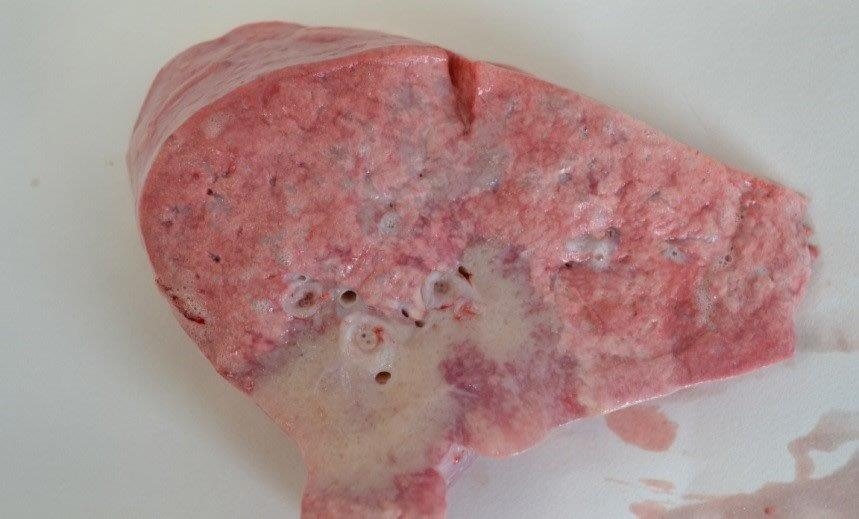
\includegraphics[width=11.93in]{_images/Jaagsiekte} 

}

\caption{Lung section demonstrating ovine pulmonary adenomatosis (Jaagsiekte). Photo:AFBI}\label{fig:foo}
\end{figure}

\subsection{Poisoning}\label{poisoning}

Copper and \emph{Pieris spp} (Forest Flame) were the most commonly
diagnosed causes of poisoning in sheep in Northern Ireland in 2017.

\begin{table}

\caption{\label{tab:unnamed-chunk-89}The  most frequently diagnosed causes of poisoning on *post-mortem* examination of sheep by AFBI during 2017 (n= 22 )}
\centering
\begin{tabular}[t]{l|r|r}
\hline
Disease & No. of cases & Percentage of total diagnoses\\
\hline
Pieris & 14 & 2.5\\
\hline
Copper & 4 & 0.7\\
\hline
Other plant poisoning & 2 & 0.4\\
\hline
Rhododendron & 2 & 0.4\\
\hline
\end{tabular}
\end{table}

\subsection{Parasitic Disease}\label{parasitic-disease}

In 2017 levels of rainfall during the months of June through to
September were considerably higher than the Northern Ireland average.
July and September saw a 60 \% increase in the level of rainfall above
normal, with June and August seeing 12\% and 33\% increase respectively.
With these conditions, the ground remained damp throughout the summer,
ideal for the survival of the intermediate host of the liver fuke, the
snail \emph{Galba truncatula}.

Although in May and June the mean monthly temperatures were higher than
the Northern Ireland average, the mean temperature for the period July
to September, at 13.2˚C, was 0.5 ˚C lower than average. Mean
temperatures of 10˚C or higher are necessary both for the breeding of
the intermediate host, the snail \emph{Galba truncatula}, and for the
development of fluke to occur within the snail. A temperature of 10˚C is
also the minimum at which fluke eggs will develop and hatch. The risk of
liver fluke infection in autumn / winter 2017 was therefore assessed by
AFBI as being particularly high especially in poorly drained areas.

\begin{table}

\caption{\label{tab:unnamed-chunk-92}The most frequently diagnosed parasitic conditions on *post-mortem* examination of sheep carcasses during 2017 (n= 188 )}
\centering
\begin{tabular}[t]{l|r|r}
\hline
Disease & No. of cases & Percentage of total diagnoses\\
\hline
Parasitic gastroenteritis & 69 & 12.3\\
\hline
Chronic fasciolosis & 50 & 8.9\\
\hline
Coccidiosis & 24 & 4.3\\
\hline
Nematodirosis & 24 & 4.3\\
\hline
Acute fasciolosis & 21 & 3.8\\
\hline
\end{tabular}
\end{table}

\subsection{Metabolic}\label{metabolic}

\begin{table}

\caption{\label{tab:unnamed-chunk-96}The most frequently diagnosed metabolic on *post-mortem* examinations of sheep carcases during 2017 (n= 23 )}
\centering
\begin{tabular}[t]{l|r|r}
\hline
Disease & No. of cases & Percentage of total diagnoses\\
\hline
Acidosis & 10 & 1.8\\
\hline
Twin lamb disease & 7 & 1.2\\
\hline
Hypocalcaemia & 3 & 0.5\\
\hline
Pregnancy toxaemia & 2 & 0.4\\
\hline
Hypomagnesaemia & 1 & 0.2\\
\hline
\end{tabular}
\end{table}

\subsection{Enteritis}\label{enteritis}

\begin{table}

\caption{\label{tab:unnamed-chunk-99}The most frequently diagnosed causes of enteritis on *post-mortem* examination of sheep carcasses during 2017 (n= 158 )}
\centering
\begin{tabular}[t]{l|r|r}
\hline
Disease & No. of cases & Percentage of total diagnoses\\
\hline
Parasitic gastroenteritis & 69 & 12.3\\
\hline
Coccidiosis & 24 & 4.3\\
\hline
Nematodirosis & 24 & 4.3\\
\hline
Diarrhoea (no organism specified) & 10 & 1.8\\
\hline
Enteritis (no organism specified) & 8 & 1.4\\
\hline
Abomasitis & 6 & 1.1\\
\hline
Colibacillosis – enteric & 3 & 0.5\\
\hline
Colienteritis & 3 & 0.5\\
\hline
Cryptosporidiosis & 2 & 0.4\\
\hline
Johne’s disease & 2 & 0.4\\
\hline
Perforated intestine & 2 & 0.4\\
\hline
Watery mouth & 2 & 0.4\\
\hline
Colibacillosis enteric – K99 positive & 1 & 0.2\\
\hline
Red gut & 1 & 0.2\\
\hline
Tapeworm infestation & 1 & 0.2\\
\hline
\end{tabular}
\end{table}

\subsection{CNS}\label{cns}

\begin{table}

\caption{\label{tab:unnamed-chunk-102}The most frequently diagnosed causes of disease affecting the nervous system  on *post-mortem* examinations of sheep carcases during 2017 (n= 27 )}
\centering
\begin{tabular}[t]{l|r|r}
\hline
Disease & No. of cases & Percentage of total diagnoses\\
\hline
Listeriosis & 15 & 2.7\\
\hline
Meningitis / encephalitis & 6 & 1.1\\
\hline
Cerebrocortical necrosis & 3 & 0.5\\
\hline
Encephalitis (no organism specified) & 2 & 0.4\\
\hline
Brain hemorrhage & 1 & 0.2\\
\hline
\end{tabular}
\end{table}

\subsection{Clostridial diseases}\label{clostridial-diseases-1}

The overall pattern of clostridial disease remains similar to 2016 with
pulpy kidney disease the most commonly diagnosed clostridial disease in
Northern Ireland. Pulpy kidney disease is caused by infection with
\emph{Clostridium perfringens} type D. It is commonly identified in fast
growing lambs, typically over one month of age that are consuming high
concentrate rations, or sucking ewes which are heavy in milk.
Vaccination of the breeding flock and early vaccination of fast growing
lambs provides the best protection and the importance of vaccination
against clostridial disease in sheep flocks cannot be over-emphasised.

\begin{table}

\caption{\label{tab:unnamed-chunk-105}: The clostridial diseases most frequently diagnosed on post-mortem examinations of ovine carcases by AFBI during 2017 (n= 32 )}
\centering
\begin{tabular}[t]{l|r|r}
\hline
Disease & No. of cases & Percentage of total diagnoses\\
\hline
Pulpy kidney diseases & 23 & 4.1\\
\hline
Black disease & 4 & 0.7\\
\hline
Clostridial diseases (no other organism specified) & 3 & 0.5\\
\hline
Enterotoxaemia & 2 & 0.4\\
\hline
\end{tabular}
\end{table}

\chapter{Ovine Abortions}\label{ovine-abortions}

\begin{center}\rule{0.5\linewidth}{\linethickness}\end{center}

Foetii from 244 ovine abortions and stillbirths were examined during
2017 in Northern Ireland. (foetii from 264 abortions were examined in
2016). Significant pathogens were detected in 165 cases (67.6 \%).
Pathogens identified included Toxoplasma (74 cases, 30.3 \%),
\emph{Chlamydophilia abortus} (44 cases, 18.0 \%), \emph{E. coli} (20
cases, 8.2 \%), \emph{Campylobacter spp} (12 cases 4.9\%),
\emph{Streptococcus spp} (9 cases, 3.7 \%), \emph{Leptospira} (8 cases,
3.3 \%), \emph{Trueperella pyogenes} (5 cases, 2.0\%) and
\emph{Listeria} (5 cases, 2.0 \%). \emph{Toxoplasma} continues to be the
most commonly diagnosed pathogen despite vaccination being widely
available. Susceptible sheep are infected following the ingestion of
feed or water contaminated with oocysts which are highly resistant and
can survive for long periods in moist conditions. Infection early in
gestation can result in foetal death and resorption, whilst infection
late in gestation can result in lambs being born normal and immune.
However infection in mid gestation can result in still born lambs, weak
lambs and mummified foetuses.

\begin{table}

\caption{\label{tab:unnamed-chunk-110}The most frequently diagnosed causes of ovine abortion diagnosed at AFBI in 2017}
\centering
\begin{tabular}[t]{l|r|r}
\hline
Category & No. of cases & Percentage\\
\hline
Toxoplasma gondi & 74 & 30.3\\
\hline
No significant agent identified. & 67 & 27.5\\
\hline
Chlamydophilia abortus & 44 & 18.0\\
\hline
E.coli & 20 & 8.2\\
\hline
Campylobacter spp & 12 & 4.9\\
\hline
Streptococcus spp & 9 & 3.7\\
\hline
Leptospirosis & 8 & 3.3\\
\hline
Arcanobacter pyogenes & 5 & 2.0\\
\hline
Listeria monocytogenes & 5 & 2.0\\
\hline
\end{tabular}
\end{table}

\begin{figure}

{\centering 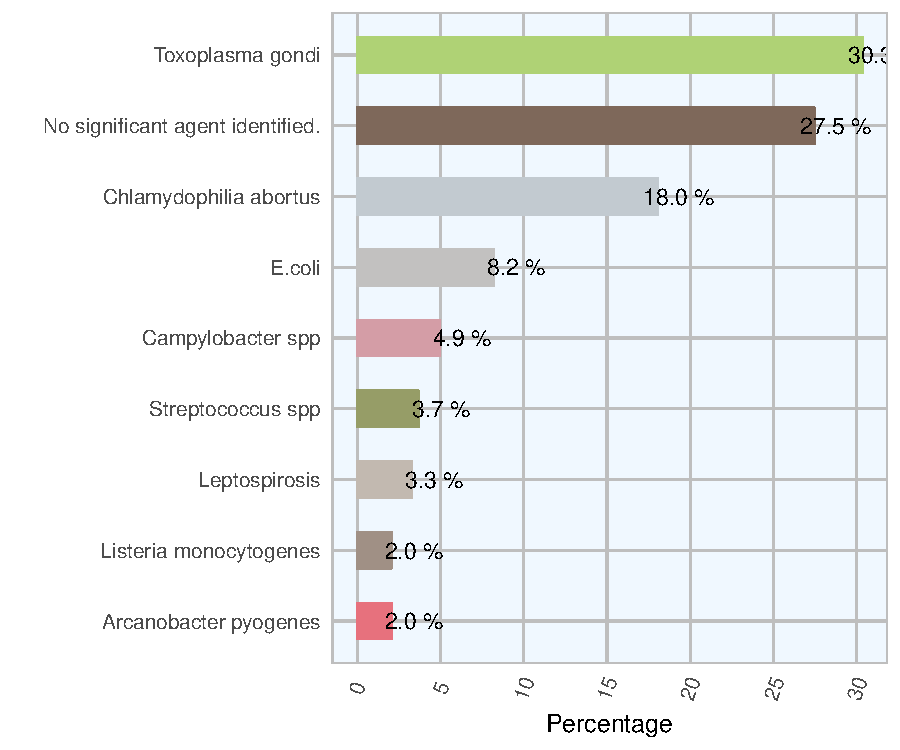
\includegraphics{AFBI_files/figure-latex/unnamed-chunk-111-1} 

}

\caption{The most frequently diagnosed causes of ovine abortion diagnosed at AFBI in 2017}\label{fig:unnamed-chunk-111}
\end{figure}

\chapter{Ovine Parasites}\label{ovine-parasites}

\begin{center}\rule{0.5\linewidth}{\linethickness}\end{center}

\section{Strongyle eggs}\label{strongyle-eggs}

\begin{figure}

{\centering 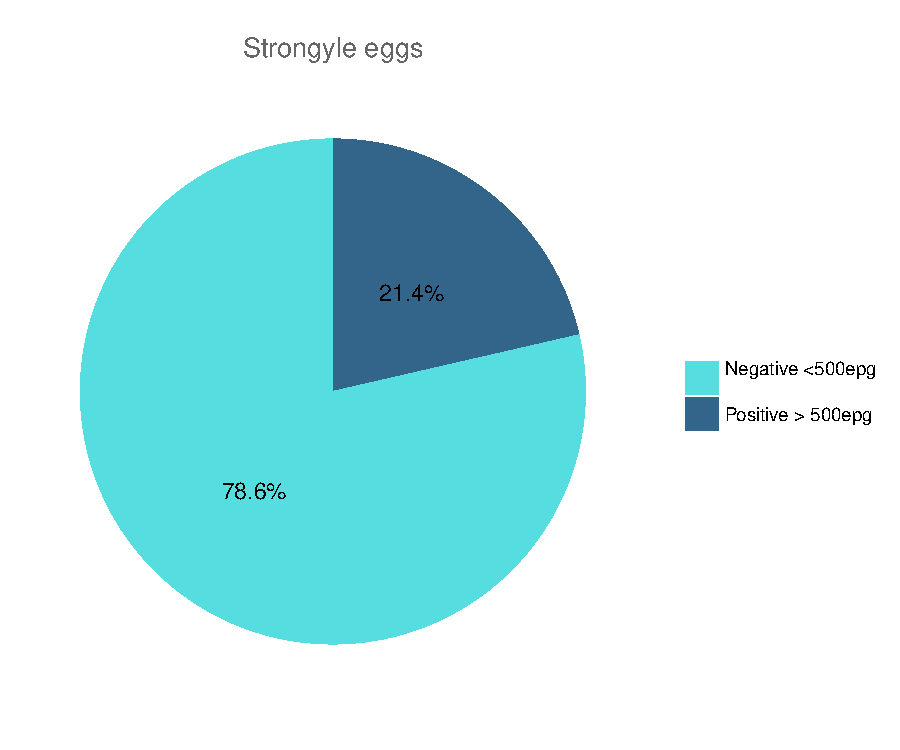
\includegraphics{AFBI_files/figure-latex/unnamed-chunk-113-1} 

}

\caption{Relative frequency of detection of trichostrongyle eggs in ovine faecal samples examined in AFBI in 2017in relation to a commonly used threshold of significance- 500 eggs per gram (n=1877)}\label{fig:unnamed-chunk-113}
\end{figure}

\section{\texorpdfstring{\emph{Nematodirus}}{Nematodirus}}\label{nematodirus}

\begin{figure}

{\centering 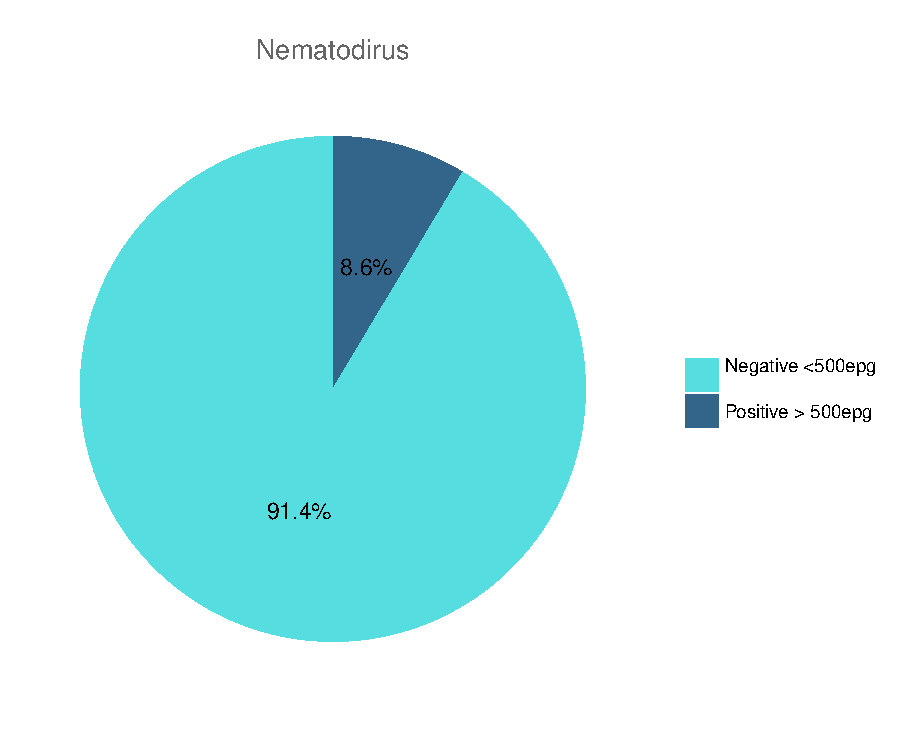
\includegraphics{AFBI_files/figure-latex/unnamed-chunk-115-1} 

}

\caption{Relative frequency of detection of *Nematodirus* eggs in ovine faecal samples examined in AFBI in 2017in relation to a commonly used threshold of significance- 200 eggs per gram (n=1812)}\label{fig:unnamed-chunk-115}
\end{figure}

\section{Liver fluke eggs}\label{liver-fluke-eggs-1}

\begin{figure}

{\centering 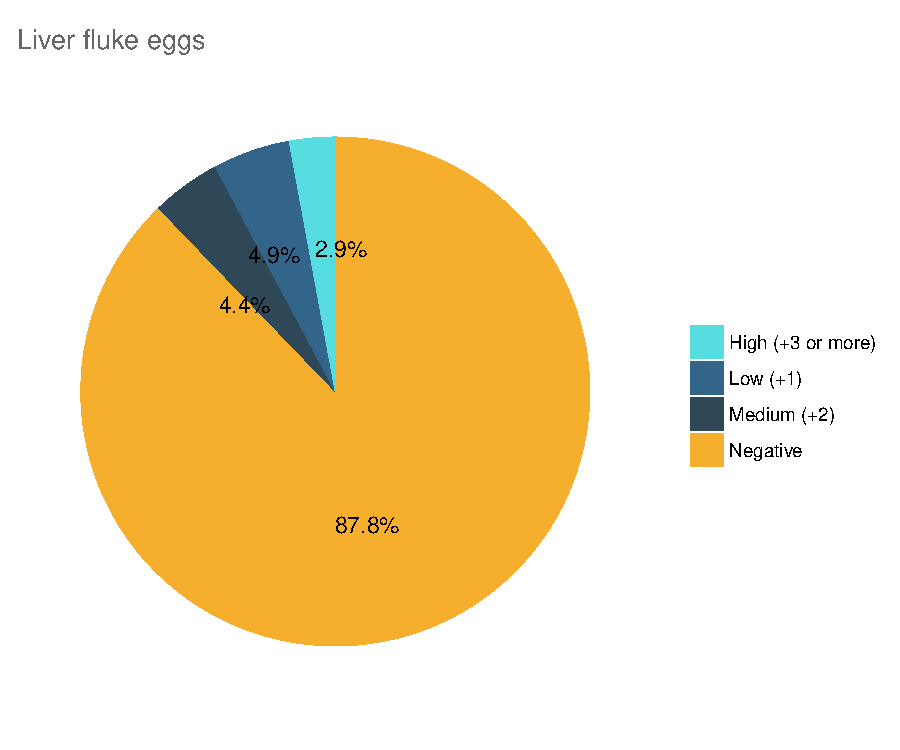
\includegraphics{AFBI_files/figure-latex/unnamed-chunk-117-1} 

}

\caption{AFBI results for ovine faecal samples tested for liver fluke eggs during 2017 (n=1781)}\label{fig:unnamed-chunk-117}
\end{figure}

\section{Rumen fluke eggs}\label{rumen-fluke-eggs-1}

\begin{figure}

{\centering 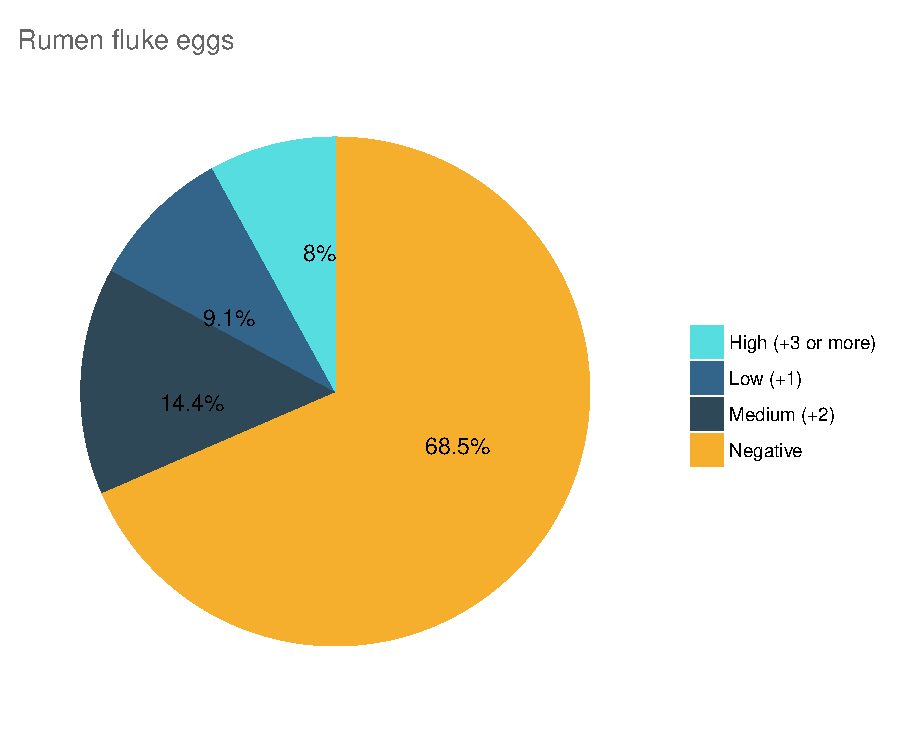
\includegraphics{AFBI_files/figure-latex/unnamed-chunk-119-1} 

}

\caption{AFBI results for ovine faecal samples tested for paramphistome eggs during 2017 (n=1780)}\label{fig:unnamed-chunk-119}
\end{figure}

\section{Coccidia}\label{coccidia-1}

\begin{figure}

{\centering 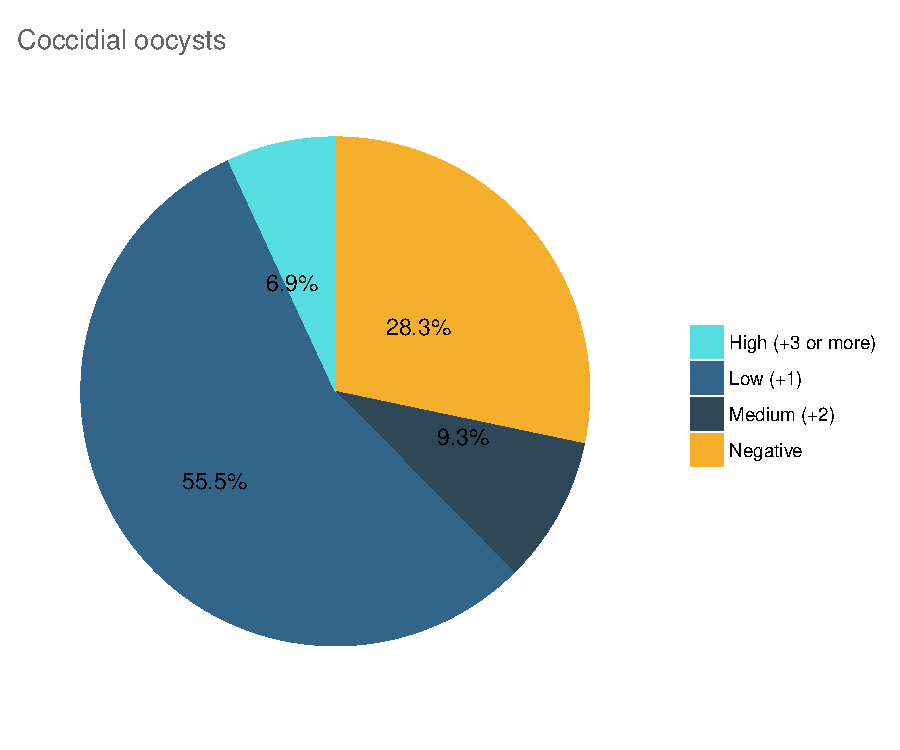
\includegraphics{AFBI_files/figure-latex/unnamed-chunk-121-1} 

}

\caption{AFBI results for ovine faecal samples tested for coccidial oocysts during 2017 (n=1882)}\label{fig:unnamed-chunk-121}
\end{figure}

\section{Timeline}\label{timeline}

\begin{figure}

{\centering 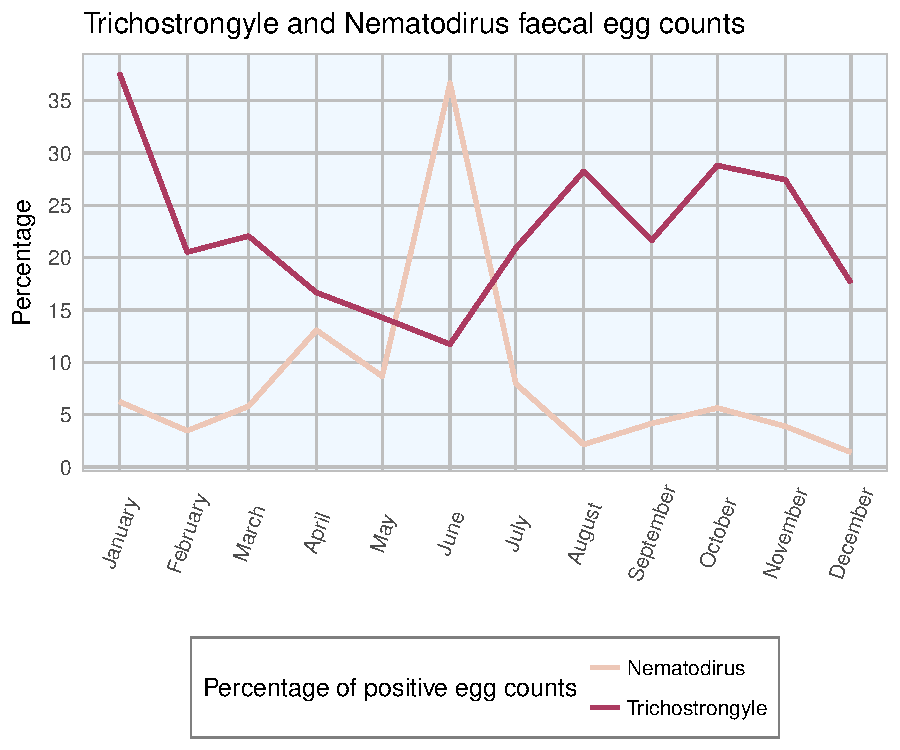
\includegraphics{AFBI_files/figure-latex/unnamed-chunk-127-1} 

}

\caption{The percentage  of ovine faecal samples tested by AFBI per month in 2017 with a Trichostrongyle egg count over 500 eggs per gram and a *Nematodirus* egg count over 200 eggs per gram}\label{fig:unnamed-chunk-127}
\end{figure}

\bibliography{book.bib,packages.bib}


\end{document}
